\documentclass[UTF8,a4paper,12pt]{ctexart}

\usepackage{geometry}
\usepackage{graphicx}
\usepackage{amsmath}
\usepackage{amssymb}
\usepackage{booktabs}
\usepackage{array}
\usepackage{tabularx}
\usepackage{longtable}
\usepackage{float}
\usepackage{xcolor}
\usepackage{listings}
\usepackage[hidelinks]{hyperref}
\usepackage{caption}
\usepackage{subcaption}
\usepackage{siunitx}

\setmonofont{Noto Sans Mono CJK SC}

\geometry{left=2.6cm,right=2.6cm,top=2.8cm,bottom=2.8cm}
\graphicspath{{figures/}}
\setlength{\parindent}{2em}
\setlength{\parskip}{0.35em}
\linespread{1.25}
\emergencystretch=3em
\newcolumntype{Y}{>{\raggedright\arraybackslash}X}
\newcolumntype{L}[1]{>{\raggedright\arraybackslash}p{#1}}
\newcommand{\codepath}[1]{\path{#1}}

\lstdefinestyle{robotcode}{
  basicstyle=\ttfamily\small,
  breaklines=true,
  breakatwhitespace=false,
  frame=single,
  columns=fullflexible,
  keepspaces=true,
  keywordstyle=\color{blue!60!black},
  commentstyle=\color{green!40!black},
  stringstyle=\color{red!50!black},
  showstringspaces=false,
  numbers=left,
  numberstyle=\tiny\color{gray},
  xleftmargin=2em,
  framexleftmargin=1.5em,
  literate={≈}{{$\approx$}}1
           {π}{{$\pi$}}1
           {τ}{{$\tau$}}1
           {α}{{$\alpha$}}1
           {θ}{{$\theta$}}1
           {↔}{{$\leftrightarrow$}}1
           {∈}{{$\in$}}1
           {≥}{{$\geq$}}1
           {℃}{{$^\circ$C}}2
           {⚠}{{\textbf{!}}}1,
  postbreak=\mbox{\textcolor{gray}{$\hookrightarrow$}\space},
  aboveskip=0.8em,
  belowskip=0.8em
}
\lstdefinestyle{appendixcode}{
  style=robotcode,
  basicstyle=\ttfamily\scriptsize,
  numberstyle=\tiny\color{gray},
  xleftmargin=1.2em,
  framexleftmargin=1em,
  aboveskip=0.6em,
  belowskip=0.6em
}
\lstset{style=robotcode}

\title{\textbf{机器人驱动与控制实验小组报告}}
\author{
  小组成员：王哲雄，王鹏远
}
\date{日期：2026 年 6 月 23 日}

\begin{document}

\maketitle
\thispagestyle{empty}
\newpage

\pagenumbering{Roman}
\tableofcontents
\newpage

\pagenumbering{arabic}

\section*{摘要}
\addcontentsline{toc}{section}{摘要}

本文围绕本学期机器人综合实验展开，按照“环境配置、运动学建模、轨迹控制、抓取搬运、相机标定、视觉定位抓取、YOLO 目标识别”的技术路线，整理了六组实验的实验目的、理论基础、程序实现、实验过程与结果分析。实验对象为六自由度桌面机械臂，软件环境基于 Python、Robotics Toolbox、OpenCV 与 YOLO 相关工具链，硬件控制通过串口转 CAN 总线完成。

通过前半部分实验，完成了机械臂开发环境配置、DH 参数建模、正逆运动学验证以及末端直线轨迹规划；通过中间实验，实现了基于关键位姿序列的物体抓取与搬运；通过后半部分实验，完成相机内参与工作空间坐标转换标定，并分别采用颜色分割与 YOLO 检测方法实现视觉引导抓取。最终实验形成了从机械臂基础运动控制到视觉感知闭环抓取的完整流程。

\textbf{关键词：} 六自由度机械臂；DH 参数；轨迹规划；相机标定；颜色识别；YOLO；视觉抓取

\newpage

\section{实验一：开发环境配置}

\subsection{实验目的}

本实验的目标是完成机械臂综合实验的软件环境整理，为后续运动控制、视觉感知和抓取程序提供统一的仿真与代码运行基础。环境配置包括 Python 依赖、机械臂串口通信方式说明、仿真模型文件、实验代码目录和安全运行约束；本组未连接真实机械臂验证硬件通信。

\subsection{软件环境}

本实验仓库根目录提供了 \texttt{environment.yml}，用于创建名为 \texttt{robot} 的 conda 环境。环境中 Python 版本为 3.10.20，主要依赖包括：

\begin{table}[H]
  \centering
  \caption{实验环境主要软件依赖}
  \small
  \begin{tabularx}{\textwidth}{L{2.3cm}Y Y}
    \toprule
    类别 & 软件包 & 用途 \\
    \midrule
    机器人建模 & \texttt{roboticstoolbox-python}, \texttt{spatialmath-python} & DH 建模、正逆运动学、轨迹规划 \\
    数值计算 & \texttt{numpy}, \texttt{scipy}, \texttt{modern-robotics} & 矩阵计算、优化求解 \\
    视觉处理 & \texttt{opencv-python}, \texttt{opencv-contrib-python} & 相机标定、颜色分割、图像显示 \\
    仿真与显示 & \texttt{matplotlib}, \texttt{pybullet}, \texttt{trimesh} & 轨迹可视化、模型检查 \\
    深度学习 & \texttt{torch}, \texttt{torchvision} & YOLO 训练和推理基础 \\
    通信控制 & \texttt{pyserial} & 串口转 CAN 通信 \\
    \bottomrule
  \end{tabularx}
\end{table}

首次配置时可在仓库根目录执行：

\begin{lstlisting}[language=bash,caption={conda 环境创建命令}]
conda env create -f environment.yml
conda activate robot
\end{lstlisting}

后续运行实验脚本时，应优先在 \texttt{daran/} 或其子目录下执行，以保证相对路径中的模型文件、字体文件和标定结果可以正确加载。

\subsection{环境配置原则}

机器人综合实验的环境配置与普通 Python 项目不同，原因在于本实验同时依赖数值计算库、机器人运动学库、相机视觉库、图形界面库以及真实串口设备。若某一类依赖版本不一致，问题往往不会立刻表现为导入失败，而是表现为仿真窗口无法打开、相机标定结果无法保存、机械臂模型姿态异常或真实关节无法通信。因此本实验采用“一套环境、一套模型、一套路径约定”的配置原则。

第一，所有 Python 代码统一运行在 \texttt{robot} 环境中。该环境同时包含 \texttt{roboticstoolbox-python}、\texttt{spatialmath-python}、\texttt{opencv-contrib-python}、\texttt{pyserial} 和 \texttt{torch} 等包，能够覆盖从 DH 建模、轨迹规划到视觉识别的主要需求。第二，所有实验脚本尽量从 \texttt{daran/} 内部运行，因为机械臂模型、字体、标定结果和图像数据大量使用相对路径。第三，涉及真实机械臂的程序必须显式区分仿真模式和实机模式，避免在检查代码或生成图像时误触发硬件动作。

从依赖来源看，\texttt{environment.yml} 使用清华镜像和 conda-forge 作为主要 channel，并将部分机器人库和视觉库通过 pip 安装。这样做可以减少课程实验中常见的二进制包冲突问题。尤其是 \texttt{roboticstoolbox-python} 依赖的 \texttt{spatialgeometry}、\texttt{swift-sim}、\texttt{rtb-data} 等包需要保持兼容，否则 DH 模型可视化和轨迹动画可能出现运行时错误。

\subsection{硬件连接与安全约束}

机械臂通过串口转 CAN 模块与上位机通信，默认波特率为 115200。代码中常见串口名称包括 Windows 下的 \texttt{COM4}/\texttt{COM7}，Linux 或 Jetson 下的 \path{/dev/ttyUSB0}，以及部分脚本中使用的 \path{/dev/serial/by-id/...}。由于 \texttt{arm\_robot} 对象在实例化后会打开串口并控制真实硬件，实验中必须区分仿真脚本和实机脚本。

本仓库采用“先仿真、后实机”的安全模式。以任务 1 和任务 2 为例，脚本中使用 \texttt{MOVE\_REAL\_ROBOT} 或人工确认按钮控制是否下发真实动作；在未来打开实机开关前，需要先检查关节限位、桌面高度、目标点可达性和仿真动画。本报告仅分析该安全设计并运行仿真，不进入实机状态。

从实验安全角度看，环境配置并不是简单的软件安装步骤，而是后续所有实验的前置保护条件。若 Python 环境、串口设备名、机械臂模型参数或标定文件路径不一致，同一段运动程序可能出现仿真正常而实机异常的情况。因此本实验首先确认依赖版本、目录结构和执行入口，并明确区分仿真验证与真实指令下发；真实硬件链路留待后续单独验证。

代码中的真实机械臂控制链路可以分为四层：最底层为串口转 CAN 通信，中间层为单关节角度与属性读写，上层为六轴机械臂的正逆运动学和夹爪控制，最外层为实验脚本中的任务流程。本次仅确认相关模块和接口的代码组织，没有验证串口设备、关节反馈或真实动作。后续若开展实机实验，应先读取关节角、显示仿真姿态并发送低速小幅目标确认通信状态，再考虑执行完整任务。

\subsection{仓库结构与实验代码组织}

实验代码主要位于 \texttt{daran/} 目录下。核心机械臂控制代码采用逐层继承结构：底层 \texttt{DrEmpower\_can.py} 负责串口/CAN 协议，\texttt{arm\_six\_axis.py} 实现六轴运动学，\texttt{gripper.py} 添加夹爪控制，\texttt{arm\_robot.py} 提供面向实验脚本的机械臂控制接口。

上述继承关系决定了后续实验的代码阅读顺序。若只关注实验脚本，可以从 \texttt{arm\_robot} 的 \texttt{set\_arm\_joints}、\texttt{read\_joints} 和夹爪接口入手；若需要解释运动学，则应回到 \texttt{arm\_six\_axis.py} 或 DH notebook；若需要分析真实执行异常，则要查看 \texttt{DrEmpower\_can.py} 中的串口通信和关节属性轮询。报告正文主要讨论实验层面的流程，但在解释误差来源时，需要同时考虑底层通信、运动学模型和执行机构三方面因素。

与本报告六个实验对应的主要文件如表 \ref{tab:repo-map} 所示。

\begin{table}[H]
  \centering
  \caption{实验内容与仓库文件对应关系}
  \label{tab:repo-map}
  \small
  \begin{tabularx}{\textwidth}{L{2.2cm}Y Y}
    \toprule
    实验 & 主要目录或文件 & 内容 \\
    \midrule
    环境配置 & \path{environment.yml}, \path{CLAUDE.md} & 环境、依赖、运行约束 \\
    直线运动 & \path{daran/task1/} & DH 建模、IK、直线轨迹仿真 \\
    抓取搬运 & \path{daran/task2/pick_and_place.py} & 示教点回放和夹爪控制 \\
    相机标定 & \path{daran/task3/camera_calibration.py} & 棋盘格内参标定 \\
    颜色视觉抓取 & \path{daran/task3/visual_grasp.py}, \path{daran/color_pick_place/} & 颜色检测、坐标转换、抓取规划 \\
    YOLO 视觉抓取 & \path{daran/color_pick_place/yolo/} & 数据集、训练、推理与接口复用 \\
    \bottomrule
  \end{tabularx}
\end{table}

\subsection{配置验证步骤}

环境配置完成后，本次从软件依赖、模型加载和运行安全三个层面进行检查。首先进入 \texttt{robot} 环境，检查 \texttt{numpy}、\texttt{roboticstoolbox}、\texttt{cv2}、\texttt{torch} 等核心包；其次运行只涉及模型和图形显示的脚本，检查 DH 模型、关节限位和仿真输出；最后阅读涉及串口控制的脚本，确认真实执行需要人工切换或按钮确认，但不连接硬件。

本实验采用的流程是“先静态检查，再仿真运行，硬件连接留待后续”。静态检查用于发现缺包、路径错误和配置文件缺失；仿真运行用于检查机械臂模型与轨迹生成逻辑。本组没有进行串口可用性、通信参数或真实关节动作验证，因此相关内容只能作为后续实机测试方案。

配置验证还包括对路径和输出文件的检查。例如任务 1 的仿真图片位于 \path{daran/task1/}，任务 2 的示教点位于 \path{daran/task2/ref_pose.json}，任务 3 的相机标定结果位于 \path{daran/task3/calibration_output/}。这些文件不仅是程序运行产物，也是报告撰写中的实验依据。如果路径不一致，后续章节中引用的图像、表格和误差指标都会失去来源。

\begin{table}[H]
  \centering
  \caption{环境配置后的验证项目}
  \label{tab:env-checklist}
  \small
  \begin{tabularx}{\textwidth}{L{2.6cm}Y Y}
    \toprule
    验证项目 & 检查内容 & 通过标准 \\
    \midrule
    Python 环境 & \texttt{robot} 环境、Python 3.10、核心包导入 & 依赖无缺失，导入不报错 \\
    DH 模型 & \texttt{RevoluteDH} 参数、关节限位、零位和 park 姿态 & 模型姿态与预期一致，坐标轴显示正常 \\
    图形输出 & matplotlib/PyPlot 后端、中文字体、GIF 或 PNG 保存 & 仿真图像能生成并保存到实验目录 \\
    相机与图像 & OpenCV 读取图像、棋盘格检测、标定文件保存 & 能检测角点并生成 JSON/NPZ 结果 \\
    串口通信 & 设备端口、波特率、关节读取接口 & 本次未连接硬件，后续需单独验证 \\
    \bottomrule
  \end{tabularx}
\end{table}

\subsection{环境复现与常见问题}

为了使报告中的实验能够被复现，环境记录不能只写“安装 Python 和 OpenCV”。本实验中较关键的版本包括 Python 3.10.20、\texttt{numpy} 1.26.4、\texttt{opencv-python} 4.11.0.86、\texttt{roboticstoolbox-python} 1.1.1、\texttt{spatialmath-python} 1.1.16、\texttt{pyserial} 3.5 和 \texttt{torch} 2.11.0。机器人建模、相机标定和 YOLO 推理分别依赖这些包的不同部分，因此版本漂移可能在不同实验中表现出不同问题。

实际配置中最常见的问题有三类。第一类是图形后端问题，例如 PyQt 与系统 Qt 库版本冲突，表现为 GUI 无法启动或出现 \texttt{xcb} 相关错误。任务 1 的 GUI 程序中加入了清理系统 \texttt{LD\_LIBRARY\_PATH} 后重启进程的逻辑，就是为了解决这类问题。第二类是路径问题，例如从仓库根目录运行脚本时找不到 \texttt{arm\_robot.py}、字体或标定文件。第三类是真实设备问题，例如串口名称变化、权限不足或 CAN 设备未连接。前两类问题可以通过静态检查和仿真验证发现，第三类必须在实机连接阶段谨慎确认。

在课程实验报告中写清这些问题有两个作用。一方面，它能解释为什么同一套代码在不同机器上可能出现不同表现；另一方面，它能说明实验设计中为什么反复强调 dry-run、仿真预览和人工确认。机器人实验的可靠性不只来自算法正确，也来自运行环境、执行入口和安全流程的一致。

\subsection{实验结果与小结}

通过环境配置实验，整理了 conda 环境、核心依赖、机械臂控制接口和实验目录结构。后续程序均基于同一个 \texttt{robot} 环境和同一套机械臂模型参数进行代码分析与仿真。安全方面，本报告只讨论不触发真实硬件动作的仿真和程序逻辑；涉及真实机械臂的脚本仅作为实现材料，未验证其硬件运行效果。

本实验也明确了后续章节的共同约束：运动控制程序应先在 DH 模型中检查关节限位和桌面高度；抓取搬运程序应先检查参考点的安全性；视觉程序应先确认相机内参、外参和坐标转换文件存在。也就是说，环境配置不是孤立的第一步，而是整套仿真与代码验证流程的入口；实机效果仍需在硬件条件具备后另行测试。

\section{实验二：机械臂末端直线运动控制}

\subsection{实验目的}

本实验要求控制机械臂末端沿笛卡尔空间中的一条直线运动。实验重点是建立机械臂 DH 模型，利用正运动学得到末端位姿，通过笛卡尔插补生成直线路径，并对路径上的每个采样点进行逆运动学求解，最终得到连续的关节角轨迹。

\subsection{机械臂运动学模型}

实验采用标准 DH 参数建立六自由度机械臂模型。模型在 \path{daran/task1/dh_cartesian_line_motion.ipynb}、\path{daran/task2/pick_and_place.py} 和 \path{daran/task3/visual_grasp.py} 中保持一致，均由 \texttt{roboticstoolbox} 的 \texttt{DHRobot} 和 \texttt{RevoluteDH} 构造。

\begin{table}[H]
  \centering
  \caption{机械臂标准 DH 参数表}
  \label{tab:dh-params}
  \small
  \begin{tabularx}{\textwidth}{L{1.5cm}YYYY}
    \toprule
    关节 & $a_i$/m & $\alpha_i$/rad & $d_i$/m & $\theta_i$ \\
    \midrule
    1 & 0 & $\pi/2$ & 0 & $q_1$ \\
    2 & 0.15 & 0 & 0 & $q_2$ \\
    3 & 0.15 & 0 & 0 & $q_3$ \\
    4 & 0 & $\pi/2$ & -0.05494 & $q_4+\pi/2$ \\
    5 & 0 & $-\pi/2$ & 0.068 & $q_5$ \\
    6 & 0 & 0 & 0.033 & $q_6$ \\
    \bottomrule
  \end{tabularx}
\end{table}

关节角限位设置为：
\[
q_{\min}=[-160,-40,-160,-160,-180,-180]^\circ,
\quad
q_{\max}=[160,180,160,160,180,180]^\circ .
\]
在每次轨迹生成后，程序都会检查所有关节角是否位于该范围内，并检查各 DH 坐标系原点是否高于桌面安全线。

\subsection{直线轨迹规划方法}

直线运动实验的起点采用安全竖直 park 姿态：
\[
q_{\text{park}}=[0,90,0,0,0,0]^\circ .
\]
在 notebook 中，起点由正运动学得到，终点通过 \texttt{path\_end\_mm} 指定。程序调用 \path{rtb.tools.trajectory.ctraj} 在起止末端位姿之间生成笛卡尔路径，再对每个路径点使用 \texttt{ikine\_LM} 求逆运动学。为了保证关节空间轨迹连续，第 $k$ 个点的逆解会作为第 $k+1$ 个点的初值。

路径生成可概括为：
\[
T_k=\text{ctraj}(T_0,T_1,N)_k,\quad
q_k=\text{IK}(T_k,q_{k-1}) .
\]
其中 $T_k$ 为第 $k$ 个末端位姿，$q_k$ 为对应关节角，$N$ 为轨迹点数。

\subsection{程序实现}

核心程序位于 \texttt{daran/task1/dh\_cartesian\_line\_motion.ipynb}。该 notebook 的主要步骤包括：

\begin{enumerate}
  \item 使用 DH 参数和关节限位创建 \texttt{DFarm\_StdDH} 模型。
  \item 设置起点 park 姿态和终点 \texttt{path\_end\_mm}。
  \item 使用 \texttt{ctraj} 生成笛卡尔直线轨迹。
  \item 对每个轨迹点调用 \texttt{ikine\_LM} 求解关节角。
  \item 计算实际末端位置与目标点的残差。
  \item 生成末端轨迹动画和关节角变化图。
\end{enumerate}

notebook 输出显示，轨迹点数为 40，最大 IK 位置残差约为 \SI{0.636}{mm}。该误差相对桌面机械臂的操作尺度较小，说明逆运动学求解能够较好跟踪笛卡尔插补路径。

关键代码如代码 \ref{lst:exp2-code} 所示，主要体现了 DH 模型构建、\texttt{ctraj} 笛卡尔插补和逐点逆运动学求解。

\lstinputlisting[
  language=Python,
  caption={末端直线运动轨迹生成与逆运动学求解},
  label={lst:exp2-code}
]{code/exp2_cartesian_line_motion.py}

\subsection{仿真与实验结果}

图 \ref{fig:task1-target} 展示了单目标位姿仿真结果，图 \ref{fig:task1-joints} 展示了对应关节角变化曲线。仿真结果表明，机械臂可以从初始安全姿态运动到目标末端位姿，且关节角变化处于限位范围内。

\begin{figure}[H]
  \centering
  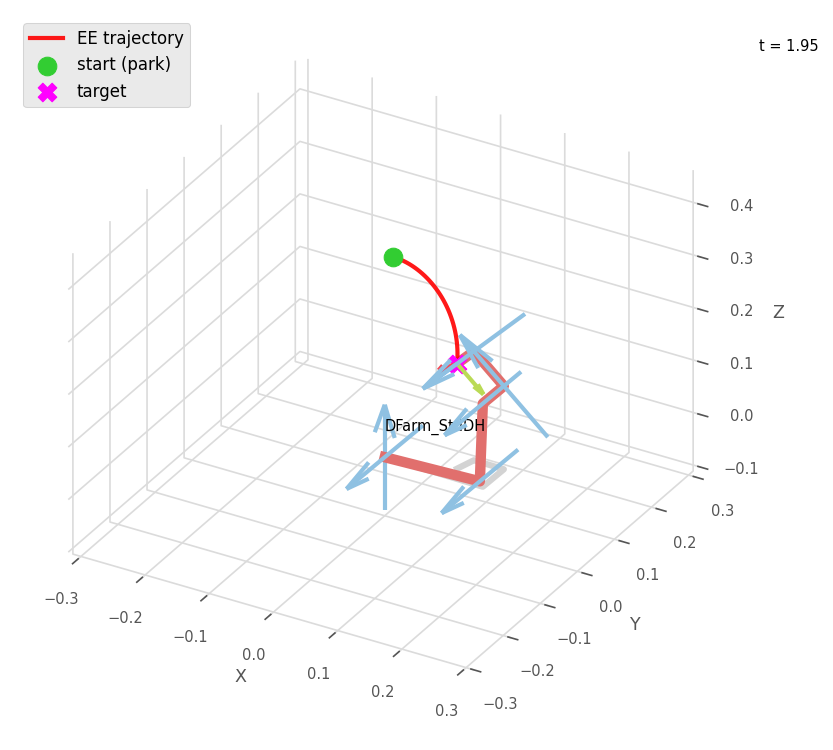
\includegraphics[width=0.78\textwidth]{task1_single_target_final.png}
  \caption{机械臂目标位姿仿真结果}
  \label{fig:task1-target}
\end{figure}

\begin{figure}[H]
  \centering
  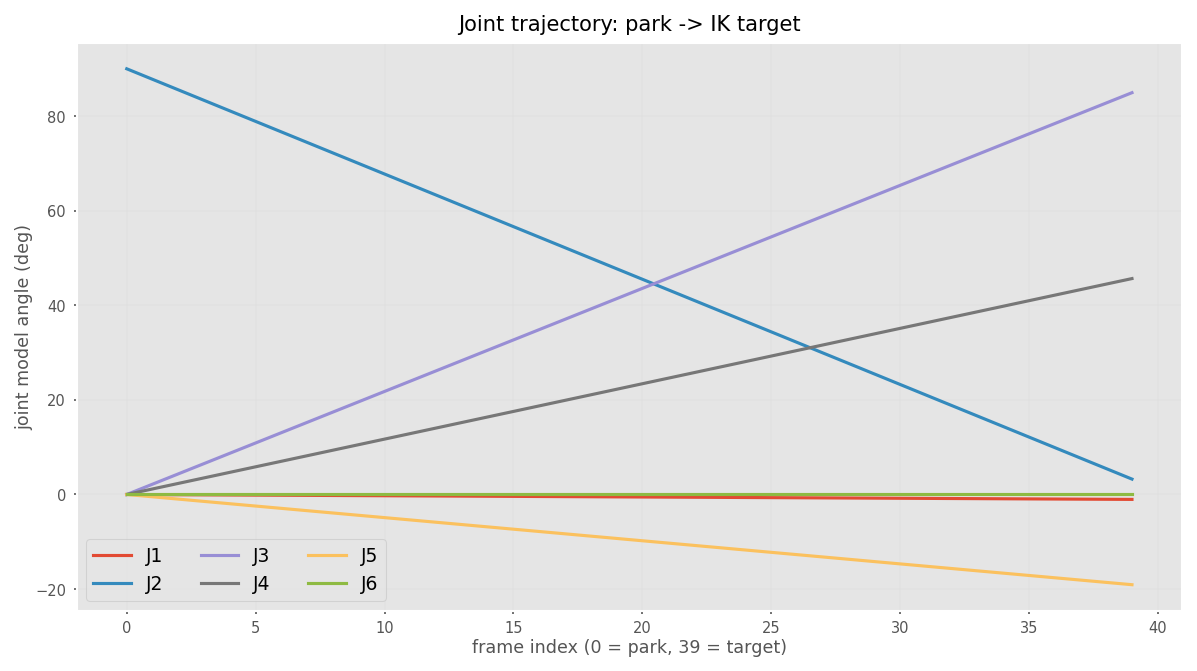
\includegraphics[width=0.78\textwidth]{task1_single_target_joints.png}
  \caption{目标运动过程中的关节角变化}
  \label{fig:task1-joints}
\end{figure}

\subsection{结果分析与小结}

本实验验证了 DH 建模、笛卡尔插补和数值逆运动学组合使用的可行性。相比直接在关节空间线性插值，笛卡尔空间插补可以更直接约束末端轨迹形状；但其代价是每个路径点都需要进行逆运动学求解，并且可能受初值、关节限位和奇异位形影响。因此程序中采用前一点解作为下一点初值，并在仿真阶段进行限位和桌面高度检查，为后续抓取搬运提供了安全的运动规划基础。

\section{实验三：机械臂抓取与搬运}

\subsection{实验目的}

本实验围绕机械臂从一点抓取物体并搬运到另一点的任务编写动作规划与仿真程序。与单纯的末端轨迹控制相比，抓取搬运程序需要同时处理关键位姿序列、夹爪开合、桌面安全高度和未来实机执行保护。

\subsection{任务流程设计}

程序位于 \path{daran/task2/pick_and_place.py}，采用参考位姿回放方式规划 A 点抓取和 B 点放置。已有文件 \path{ref_pose.json} 中记录了四个关键点：

\begin{table}[H]
  \centering
  \caption{抓取搬运实验示教点}
  \label{tab:pick-place-points}
  \small
  \begin{tabularx}{0.82\textwidth}{L{1.5cm}L{2.5cm}Y}
    \toprule
    顺序 & 名称 & 含义 \\
    \midrule
    1 & A\_safe & A 点上方安全位 \\
    2 & A\_grasp & A 点抓取位 \\
    3 & B\_safe & B 点上方安全位 \\
    4 & B\_place & B 点放置位 \\
    \bottomrule
  \end{tabularx}
\end{table}

完整执行序列为：
\[
\text{park}\rightarrow A_{\text{safe}}\rightarrow A_{\text{grasp}}\rightarrow
A_{\text{safe}}\rightarrow B_{\text{safe}}\rightarrow B_{\text{place}}\rightarrow
B_{\text{safe}}\rightarrow \text{park}.
\]
其中到达 A 点抓取位后闭合夹爪，到达 B 点放置位后打开夹爪。

该流程采用“上方安全点”和“接触操作点”分离的设计。真实机械臂在桌面附近水平移动时，夹爪或物体可能与桌面、障碍物发生干涉，因此程序规划末端先移动到目标点上方，再沿近似竖直方向下降到抓取或放置位。这个设计为后续实机实验预留了安全动作模板，但其实际避碰效果尚未验证。

\subsection{示教点记录}

\path{ref_pose.json} 中的四组参考数据包含六个机械臂关节角和夹爪角度。本组将其作为仿真输入，没有通过真实机械臂重新示教或验证。表 \ref{tab:pick-place-joints} 给出了四个关键点的模型关节角，表 \ref{tab:pick-place-fk} 给出了由 DH 正运动学计算得到的末端坐标。

\begin{table}[H]
  \centering
  \caption{抓取搬运示教点关节角}
  \label{tab:pick-place-joints}
  \small
  \begin{tabularx}{\textwidth}{L{1.6cm}YYYYYY}
    \toprule
    点位 & $q_1$ & $q_2$ & $q_3$ & $q_4$ & $q_5$ & $q_6$ \\
    \midrule
    A\_safe & 22.5 & 58.9 & -46.9 & -1.9 & 84.5 & 22.7 \\
    A\_grasp & 17.9 & 53.4 & -53.7 & 7.3 & 92.2 & 12.0 \\
    B\_safe & -24.4 & 60.9 & -50.7 & -0.6 & 83.6 & -24.8 \\
    B\_place & -23.8 & 55.6 & -57.7 & 7.2 & 82.7 & -24.9 \\
    \bottomrule
  \end{tabularx}
\end{table}

\begin{table}[H]
  \centering
  \caption{示教点正运动学末端坐标}
  \label{tab:pick-place-fk}
  \small
  \begin{tabularx}{0.78\textwidth}{L{1.8cm}YYY}
    \toprule
    点位 & $x$/mm & $y$/mm & $z$/mm \\
    \midrule
    A\_safe & 254.5 & 161.5 & 139.2 \\
    A\_grasp & 278.6 & 149.1 & 95.2 \\
    B\_safe & 288.1 & -74.4 & 136.6 \\
    B\_place & 299.8 & -76.8 & 91.7 \\
    \bottomrule
  \end{tabularx}
\end{table}

从表 \ref{tab:pick-place-fk} 可以看到，A 点安全位到抓取位的末端高度下降约 \SI{44.0}{mm}，B 点安全位到放置位的高度下降约 \SI{44.9}{mm}，均小于程序设定的 \SI{120}{mm} 下降幅度上限。同时，两个 safe 点高度均高于 \SI{130}{mm}，满足脚本中的安全高度要求。这说明示教点并非只记录目标位置，还记录了完整任务中“安全接近”和“低位接触”的空间关系。

\subsection{关键位姿与夹爪控制}

脚本定义了固定 park 位姿 $[0,90,0,0,0,0]^\circ$ 作为任务起止安全姿态。示教点中的关节角全部经过限位检查，A/B 安全点还需满足末端高度不低于 \SI{130}{mm}，safe 点到 grasp/place 点的下降幅度不得超过 \SI{120}{mm}。

夹爪控制代码未直接使用原始 \texttt{grasp()} 接口，而是根据程序中给定的换算关系调用底层 \path{set_angle_adaptive}：
\[
\theta_g = w \cdot \frac{-180}{\pi d},
\]
其中 $w$ 为夹爪开口宽度，$d=\SI{10}{mm}$ 为夹爪传动直径。程序设置的张开宽度为 \SI{6.0}{mm}，夹紧宽度为 \SI{1.8}{mm}，闭爪力参数约为 \SI{40}{N}；这些参数未在实物夹取中验证。

\subsection{实验步骤与安全检查}

抓取搬运实验首先通过示教或已有文件获得 A、B 两处关键位姿，然后由程序读取 \path{ref_pose.json} 并进行格式检查。随后程序根据 DH 模型计算各示教点的末端高度，确认 safe 点高于桌面安全线，且从 safe 点下降到 grasp/place 点的距离处于允许范围内。只有在这些检查通过后，程序才会生成完整动作序列。

仿真阶段主要观察三类现象：第一，机械臂是否能从 park 姿态平滑到达各关键点；第二，下降和抬升动作是否基本沿竖直方向进行；第三，关节角是否存在突变或接近限位的情况。实机执行阶段则需要额外确认夹爪开口是否与物体尺寸匹配，目标物体是否位于示教抓取点附近，以及抓取后物体是否会因重心偏移而滑落。

程序将 10 个任务步骤组织为统一计划，其中 7 个为机械臂移动段，3 个为夹爪动作段。每个移动段使用五次多项式关节插值生成 40 个采样点；每个夹爪动作在仿真中用短暂停顿表示，以便观察动作时序。因此仿真轨迹不仅展示机械臂从 A 点移动到 B 点的空间路径，也展示了抓取前张爪、抓取后闭爪和放置后张爪的时序位置。

安全检查分为示教点检查和整条轨迹检查两类。示教点检查关注四个关键点本身是否合理，例如关节角是否越界、safe 点是否高于抓取点、下降距离是否过大；整条轨迹检查则关注插值过程中是否出现中间姿态低于桌面或末端高度异常。这样可以避免一种常见问题：起点和终点都安全，但两点之间的插值姿态穿过危险区域。

\subsection{程序实现}

抓取搬运程序沿用了实验二中的 DH 模型和关节限位。主要函数包括：

\begin{itemize}
  \item \texttt{load\_waypoints()}：读取示教点并检查数据长度和关节限位。
  \item \texttt{safety\_check\_reference\_set()}：计算示教点正运动学位置，检查桌面高度、安全点高度和下降幅度。
  \item \texttt{build\_plan()}：构造移动和夹爪动作序列。
  \item \texttt{verify\_ee\_z\_floor()}：检查整条轨迹末端高度下限。
  \item \texttt{MOVE\_REAL\_ROBOT}：控制是否真实下发串口指令。
\end{itemize}

值得注意的是，脚本头部注释要求先将 \texttt{MOVE\_REAL\_ROBOT} 设为 \texttt{False} 生成仿真动画，再由操作者决定是否进入实机模式。本组始终保持仿真模式，没有将动作下发到真实机械臂。

为未来实机执行，代码没有直接使用库中无超时的 \texttt{pose\_done()} 或 \texttt{grasp\_done()} 轮询，而是实现了带超时的等待函数。其设计目标是在关节未按时到位时中止任务，并区分张爪故障与闭爪接触物体两类情况。由于本组未连接硬件，这些超时与接触判断逻辑仅完成代码检查，尚未验证实际行为。

抓取搬运的核心动作序列和夹爪宽度到角度的换算如代码 \ref{lst:exp3-code} 所示。代码中将移动动作和夹爪动作放在同一计划列表中，便于仿真和实机执行共用同一套流程。

\lstinputlisting[
  language=Python,
  caption={抓取搬运动作序列与夹爪宽度换算},
  label={lst:exp3-code}
]{code/exp3_pick_and_place.py}

\subsection{仿真结果与分析}

图 \ref{fig:task3-pick-place} 为抓取搬运动画中抽取的关键帧。仿真模型先回到竖直 park 姿态，再移动到 A 点上方；下降到抓取位后显示闭爪时序，随后抬升、平移至 B 点上方，再下降并显示开爪时序。该动画用于检查动作顺序和模型姿态，不代表夹爪已经接触或搬运真实物体。

\begin{figure}[H]
  \centering
  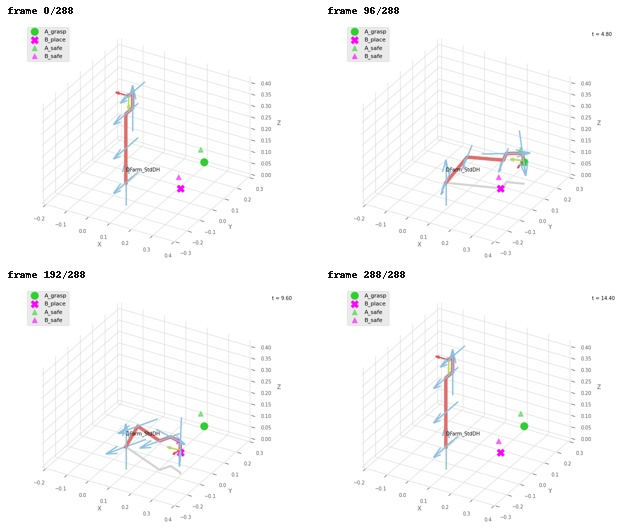
\includegraphics[width=0.82\textwidth]{task3_pick_place_keyframes.jpg}
  \caption{抓取搬运过程仿真关键帧}
  \label{fig:task3-pick-place}
\end{figure}

关键帧中可以看到，A 点和 B 点均设置 safe/grasp 或 safe/place 两级高度，模型在低位只执行短距离接近和离开动作，主要水平移动发生在安全高度附近。这与表 \ref{tab:pick-place-fk} 中 safe 点高于 grasp/place 点约 \SI{44}{mm} 的数据一致，也说明参考点不是孤立位置，而是服务于完整任务时序的空间约束。

本实验的精度主要依赖示教点质量。若 A\_grasp 点偏离物体中心，夹爪可能只夹住物体边缘；若 B\_place 点高度过低，放置时可能挤压桌面；若 safe 点高度不足，平移过程中可能带动物体碰撞其它物体。因此示教点不仅记录位置，还隐含了操作者对安全高度、抓取方向和物体尺寸的经验判断。后续视觉抓取的目标是将其中“抓取点位置”由视觉自动给出，但 safe 点构造和夹爪动作顺序仍沿用本实验的思想。

与实验二相比，本实验的核心难点不再是单条直线是否足够直，而是任务序列是否满足接触操作的约束。抓取动作必须在物体上方张爪，在接触高度闭爪，再抬升到安全高度后水平搬运；放置动作则必须在目标上方下降，松开夹爪后再抬升离开。任何一步时序错误都可能导致空抓、碰撞或拖动物体。因此本实验从运动控制上升到了任务规划层面。

从后续实机风险看，抓取搬运既包含运动学误差，也包含夹爪和物体接触误差。即使关节到达参考角度，如果物体位置与参考抓取点存在偏差，夹爪仍可能抓偏；夹爪力过小可能导致滑落，过大则可能挤压物体。任务 2 中的夹爪宽度、闭爪力和停顿时间目前只是程序参数，需通过实物实验重新调整。

\subsection{失败模式与保护策略}

抓取搬运任务比单纯运动控制更容易失败，因为它涉及机械臂、夹爪、物体和桌面之间的接触。根据程序结构可以预判四类失败模式。第一类是参考点错误，例如 A\_grasp 没有对准物体中心，或 B\_place 过低；第二类是轨迹错误，例如 safe 点高度不足；第三类是夹爪错误，例如张爪不到位或闭爪力不足；第四类是通信和执行错误，例如关节未按时到位或串口读取失败。这些模式尚未通过本组实物实验观察。

脚本中的保护策略正是围绕这些失败模式展开。参考点错误通过关节限位、safe 高度和下降幅度检查发现；轨迹错误通过整条插值轨迹的桌面高度扫描发现；夹爪与执行错误则预期通过宽度反馈轮询、关节到位轮询、超时和异常中止处理。这些保护逻辑是否能够覆盖真实机械臂故障仍需后续测试。

需要注意的是，保护策略只能降低风险，不能消除所有风险。例如程序可以检查末端坐标系高度，但无法直接知道夹爪外形、物体实际高度和桌面上其它障碍物的位置；程序可以等待关节到位，但无法完全判断物体是否已经被稳定夹住。因此实机执行前仍然需要操作者观察仿真动画、清理工作区、确认物体位置，并在任务运行时保持可中止状态。

\subsection{小结}

本实验在代码和仿真中将前一实验的轨迹规划扩展为包含夹爪动作的任务级流程。其关键不是单个点的运动，而是多个安全位姿之间的顺序约束。后续视觉抓取程序也是先通过视觉确定抓取点，再生成类似的 safe-grasp-safe 序列，因此本实验为视觉抓取提供了动作模板。

本实验也暴露了示教回放方法的局限性：它要求物体每次都放在相同位置，且放置点环境不能发生明显变化。一旦物体初始位置偏移，固定示教点就无法自动修正。因此实验四和实验五继续引入相机标定与视觉定位，使系统能够由图像实时确定目标位置，从而把本实验中的固定 A\_grasp 点替换为视觉计算得到的抓取点。

\section{实验四：相机标定}

\subsection{实验目的}

本实验目标是整理相机内参、畸变参数以及相机与工作平面之间位姿关系的计算流程，为后续从图像像素坐标推算机械臂抓取坐标提供程序基础。本组未通过真实机械臂运动检验转换后的抓取坐标。

\subsection{相机成像模型}

实验采用针孔相机模型。空间点 $P_C=[X_C,Y_C,Z_C]^T$ 在相机坐标系下投影到像素平面：
\[
s
\begin{bmatrix}
u\\v\\1
\end{bmatrix}
=
K
\begin{bmatrix}
X_C\\Y_C\\Z_C
\end{bmatrix},
\quad
K=
\begin{bmatrix}
f_x&0&c_x\\
0&f_y&c_y\\
0&0&1
\end{bmatrix}.
\]
其中 $K$ 为相机内参矩阵，$f_x,f_y$ 为像素焦距，$c_x,c_y$ 为主点坐标。实际镜头还存在径向畸变和切向畸变，需要通过标定估计畸变系数。

\subsection{内参与畸变标定}

内参标定程序为 \path{daran/task3/camera_calibration.py}。程序支持实时采集和从已有图片标定两种方式。实验使用 $7\times7$ 内角点棋盘格，方格边长为 \SI{0.008}{m}，有效标定图像共 30 张。程序流程如下：

\begin{enumerate}
  \item 使用 \texttt{cv2.findChessboardCorners} 检测棋盘格角点。
  \item 使用 \texttt{cv2.cornerSubPix} 对角点进行亚像素优化。
  \item 构造棋盘格世界坐标点。
  \item 调用 \texttt{cv2.calibrateCamera} 求解内参和畸变。
  \item 保存 \path{camera_calibration.json}、\path{camera_calibration.npz} 和去畸变示例图。
\end{enumerate}

标定结果如表 \ref{tab:camera-calib} 所示。

\begin{table}[H]
  \centering
  \caption{相机内参标定结果}
  \label{tab:camera-calib}
  \small
  \begin{tabularx}{0.72\textwidth}{L{3.5cm}Y}
    \toprule
    项目 & 数值 \\
    \midrule
    图像尺寸 & $640\times480$ \\
    有效图像数 & 30 \\
    RMS 重投影误差 & 0.2025 px \\
    平均重投影误差 & 0.2025 px \\
    $f_x$ & 381.2781 \\
    $f_y$ & 508.3521 \\
    $c_x$ & 319.2541 \\
    $c_y$ & 239.6599 \\
    \bottomrule
  \end{tabularx}
\end{table}

标定得到的相机矩阵为：
\[
K=
\begin{bmatrix}
381.2781 & 0 & 319.2541\\
0 & 508.3521 & 239.6599\\
0 & 0 & 1
\end{bmatrix}.
\]
畸变系数采用 OpenCV 默认顺序，可写为：
\[
(k_1,k_2,p_1,p_2,k_3)
=(0.1455,-0.2150,-0.0025,0.0029,0.0715).
\]
其中 $k_1,k_2,k_3$ 描述径向畸变，$p_1,p_2$ 描述切向畸变。径向畸变主要与镜头边缘区域的弯曲有关，切向畸变则与镜头和成像平面不完全平行有关。去畸变后程序还计算了新的相机矩阵
\[
K_{\text{new}}=
\begin{bmatrix}
383.3236 & 0 & 322.0648\\
0 & 509.6299 & 237.8273\\
0 & 0 & 1
\end{bmatrix},
\]
对应有效 ROI 为 $(6,6,628,466)$。这意味着去畸变图像会裁掉少量边缘区域，以减少无效黑边对后续识别的影响。

重投影误差是评价标定质量的重要指标。标定完成后，程序会将棋盘格世界坐标点通过估计得到的相机参数重新投影到图像平面，再与实际检测到的角点位置比较。若误差较小，说明内参、畸变参数和各标定图像的位姿能够较好解释观测数据。本实验平均重投影误差约为 0.2025 px，表明角点检测和内参求解具有较好一致性。

标定图像的采集质量会直接影响结果。理想情况下，棋盘格应覆盖图像中心和边缘区域，并包含不同倾角和不同距离的姿态；若图像都集中在画面中央，畸变参数约束不足；若棋盘格角点模糊、反光或遮挡，亚像素角点会产生偏差。因此相机标定不仅是一次函数调用，更依赖采集过程中的姿态多样性和图像清晰度。

标定程序中棋盘格三维点生成、角点检测和相机标定调用如代码 \ref{lst:exp4-code} 所示。该部分是后续所有像素坐标转换的基础。

\lstinputlisting[
  language=Python,
  caption={棋盘格角点检测与相机内参标定核心代码},
  label={lst:exp4-code}
]{code/exp4_camera_calibration.py}

\begin{figure}[H]
  \centering
  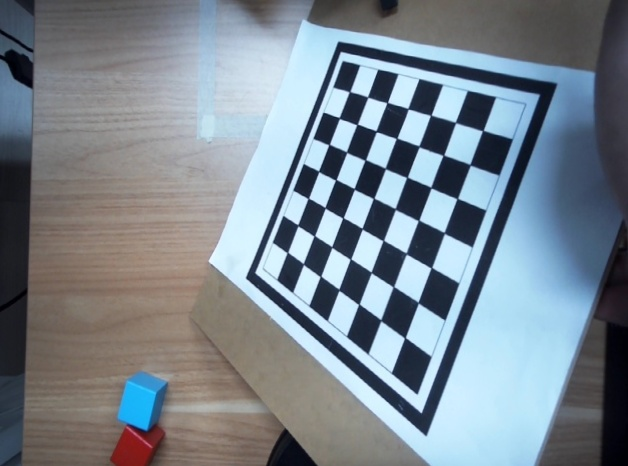
\includegraphics[width=0.72\textwidth]{task4_undistorted_example.jpg}
  \caption{相机去畸变示例图}
  \label{fig:task4-undistorted}
\end{figure}

\subsection{工作空间坐标转换}

外参估计程序为 \path{daran/task3/pose_projection.py}。在工作平面上放置棋盘格后，程序通过 \texttt{cv2.solvePnP} 求解世界坐标系到相机坐标系的变换矩阵，并保存 \path{camera_extrinsic.json}。实验得到的外参重投影误差约为 0.0215 px。

本实验中棋盘格坐标系到相机坐标系的平移向量为：
\[
t=
\begin{bmatrix}
-0.0158 & -0.0316 & 0.1572
\end{bmatrix}^T\text{m},
\]
说明棋盘格原点相对于相机光心位于约 \SI{15.7}{cm} 的深度处。旋转向量为：
\[
r=
\begin{bmatrix}
-0.0234 & -0.0160 & 0.0074
\end{bmatrix}^T,
\]
其数值较小，说明棋盘格平面相对于相机坐标系的倾斜角不大。对应的世界到相机齐次变换矩阵为：
\[
T_{C}^{W}=
\begin{bmatrix}
0.9998 & -0.0072 & -0.0161 & -0.0158\\
0.0076 & 0.9997 & 0.0233 & -0.0316\\
0.0159 & -0.0234 & 0.9996 & 0.1572\\
0 & 0 & 0 & 1
\end{bmatrix}.
\]
该矩阵的前三列描述棋盘格坐标轴在相机坐标系中的方向，最后一列描述棋盘格原点在相机坐标系中的位置。

对于一个像素点 $(u,v)$，程序先使用内参和畸变参数通过 \texttt{cv2.\allowbreak undistortPoints} 得到相机归一化射线，再将射线变换到世界坐标系，并与工作平面 $z=z_0$ 求交：
\[
P_W = O_W + \lambda d_W,\quad
\lambda = \frac{z_0-O_{W,z}}{d_{W,z}} .
\]
在视觉抓取实验中，还需要将棋盘格或相机工作平面坐标转换到机械臂基坐标。当前 \path{workspace_transform.json} 中采用的轴关系为：
\[
x_{\text{base}}=-y_{\text{cam}}+0.300,\quad
y_{\text{base}}=x_{\text{cam}}-0.028,\quad
z_{\text{base}}=z_{\text{cam}}.
\]
对应齐次矩阵为：
\[
T_{B}^{W}=
\begin{bmatrix}
0 & -1 & 0 & 0.300\\
1 & 0 & 0 & -0.028\\
0 & 0 & 1 & 0\\
0 & 0 & 0 & 1
\end{bmatrix}.
\]
这个矩阵表明，棋盘格平面坐标与机械臂基坐标之间存在一个平面内的 $90^\circ$ 轴向交换和一个平移偏置。后续视觉抓取中，目标像素中心先被反投影到棋盘格或工作平面坐标，再通过该矩阵转换到机械臂基坐标。

\begin{figure}[H]
  \centering
  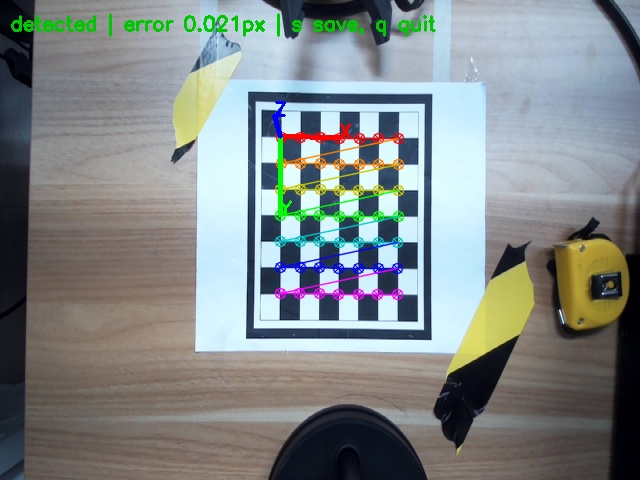
\includegraphics[width=0.72\textwidth]{task4_camera_extrinsic_preview.jpg}
  \caption{棋盘格外参估计与坐标轴投影}
  \label{fig:task4-extrinsic}
\end{figure}

\subsection{实验步骤}

本实验代码使用已有棋盘格图像并剔除角点检测失败的样本，然后运行内参标定程序生成相机矩阵和畸变系数。获得内参后，程序利用 \texttt{solvePnP} 求解棋盘格坐标系相对于相机坐标系的位姿。最后，结合工作平面高度假设，将像素点反投影成空间射线，并求出其与桌面的交点。

实验过程中需要特别注意单位一致性。棋盘格方格边长以米为单位进入内参标定和外参估计，而机械臂控制程序中部分坐标采用毫米表示；如果单位混用，坐标转换结果会出现数量级错误。为避免这一问题，报告中统一在表格和公式中标注单位，并在代码分析中区分相机坐标、棋盘格坐标和机械臂基坐标。

为了检查外参是否合理，程序在图像上绘制棋盘格角点和三维坐标轴投影。若坐标轴方向与实际棋盘格摆放方向明显不一致，说明角点顺序、方格尺寸或外参求解存在问题；若坐标轴位置正确但重投影误差偏大，则可能是图像模糊、棋盘格没有铺平或内参不准确。图 \ref{fig:task4-extrinsic} 中坐标轴能够较好贴合棋盘格角点，因此可作为后续像素反投影的基础。

\subsection{标定结果与分析}

从内参标定结果看，平均重投影误差约为 0.20 px，说明棋盘格角点拟合精度较高。外参估计的重投影误差更低，约为 0.0215 px，表明在单幅棋盘格图像上估计得到的位姿与角点观测匹配良好。

但需要注意，图像重投影误差小并不等价于机械臂抓取误差一定小。抓取误差还会受到以下因素影响：

\begin{itemize}
  \item 相机安装位置和工作平面是否稳定；
  \item 棋盘格平面与真实物体上表面是否存在高度差；
  \item 像素中心提取是否受光照、遮挡和颜色反光影响；
  \item 机械臂自身运动学模型和舵机回差误差。
\end{itemize}

从机器人抓取角度看，标定误差会沿着“像素中心、相机射线、工作平面交点、机械臂基坐标”的链路逐级传递。即使像素级重投影误差很小，只要相机外参或桌面高度假设存在偏差，最终机械臂坐标也可能产生毫米级甚至厘米级误差。因此现有重投影误差只能说明图像角点拟合情况，不能证明真实机械臂抓取坐标准确。

本实验还说明了单目相机定位的一个基本限制：单个像素点只能确定一条空间射线，不能直接确定三维坐标。只有引入工作平面高度 $z=z_0$ 之后，射线与平面的交点才成为唯一的空间点。因此本实验适合桌面色块抓取这类目标高度近似固定的场景；若目标高度变化较大，或者物体堆叠，单一平面假设就会带来明显误差。此时需要引入深度相机、多视角重建或抓取前二次视觉确认。

\subsection{标定文件在系统中的作用}

相机标定实验最终生成多个文件，它们在后续视觉抓取中的作用不同。若只保存一张去畸变图像，无法支持实时抓取；若只保存内参而没有工作空间变换，也无法将像素点转换到机械臂坐标。因此标定结果需要按用途组织，如表 \ref{tab:calib-files} 所示。

\begin{table}[H]
  \centering
  \caption{相机标定输出文件及用途}
  \label{tab:calib-files}
  \small
  \begin{tabularx}{\textwidth}{L{4.0cm}Y Y}
    \toprule
    文件 & 主要内容 & 后续用途 \\
    \midrule
    \path{camera_calibration.json} & 图像尺寸、内参矩阵、畸变系数、重投影误差 & 去畸变、像素射线计算 \\
    \path{camera_calibration.npz} & NumPy 格式内参、畸变和新相机矩阵 & 供 Python 程序快速加载 \\
    \path{undistorted_example.jpg} & 去畸变效果图 & 检查标定结果是否合理 \\
    \path{camera_extrinsic.json} & 棋盘格到相机的外参、重投影误差 & 像素点投影和反投影 \\
    \path{camera_extrinsic_preview.jpg} & 坐标轴投影预览图 & 人工检查外参方向 \\
    \path{workspace_transform.json} & 工作平面到机械臂基坐标的轴关系和平移 & 将工作平面坐标转换为抓取坐标 \\
    \bottomrule
  \end{tabularx}
\end{table}

这些文件共同构成视觉抓取的坐标基础。实验五和实验六在识别算法上不同，但都必须依赖这里的标定结果。若相机位置移动、焦距变化、分辨率改变或棋盘格坐标系重新定义，相关标定文件都需要重新生成，否则后续抓取点会系统性偏移。由此可见，相机标定并不是一次性的“前处理”，而是视觉系统稳定运行的前置条件。

\subsection{小结}

本实验整理并运行了从像素坐标到工作平面坐标的标定计算程序。后续颜色识别和 YOLO 识别都需要利用相机内参、外参和工作空间到机械臂基坐标的转换关系生成候选抓取坐标，但该坐标尚未通过真实机械臂到点实验验证。

\section{实验五：基于颜色识别的视觉抓取}

\subsection{实验目的}

本实验在相机标定代码基础上，通过颜色识别获得物体在图像中的位置，再将像素坐标转换为机械臂基坐标，并生成抓取与放置轨迹的仿真方案。相比前面的参考点回放，本实验由视觉结果计算候选抓取点，体现了从固定动作到视觉引导规划的程序结构转变；本组未执行真实抓取。

\subsection{颜色分割与目标定位}

颜色识别代码主要位于 \path{daran/color_pick_place/detect.py}。程序定义了红、绿、蓝、黄四类颜色的 HSV 阈值范围，对图像进行颜色分割后，通过轮廓提取获得候选色块。检测流程如下：

\begin{enumerate}
  \item 读取相机图像并根据标定参数进行去畸变。
  \item 将 BGR 图像转换到 HSV 颜色空间。
  \item 根据目标颜色阈值生成二值 mask。
  \item 使用开运算和闭运算去除噪声、填补孔洞。
  \item 通过 \texttt{cv2.findContours} 提取轮廓。
  \item 根据面积阈值和长宽比过滤非方块目标。
  \item 使用 \texttt{cv2.minAreaRect} 得到目标中心、边界框和旋转角。
\end{enumerate}

对于蓝色和绿色，程序还叠加了 BGR 通道约束。例如蓝色目标要求蓝色通道显著高于红色和绿色通道，以增强在复杂光照下的鲁棒性。

各颜色的 HSV 阈值如表 \ref{tab:color-thresholds} 所示。红色在 HSV 中跨越 0 度边界，因此需要使用两个区间合并；蓝色和绿色除 HSV 阈值外还加入了原始 BGR 通道约束，用于过滤偏灰或反光区域。

\begin{table}[H]
  \centering
  \caption{颜色识别 HSV 阈值设置}
  \label{tab:color-thresholds}
  \small
  \begin{tabularx}{0.88\textwidth}{L{1.6cm}Y}
    \toprule
    颜色 & HSV 范围 \\
    \midrule
    red & $[0,100,100]\sim[10,255,255]$，$[160,100,100]\sim[179,255,255]$ \\
    green & $[35,50,50]\sim[85,255,255]$ \\
    blue & $[78,70,35]\sim[135,255,255]$ \\
    yellow & $[20,100,100]\sim[30,255,255]$ \\
    \bottomrule
  \end{tabularx}
\end{table}

选择 HSV 颜色空间的原因是其将色相、饱和度和亮度近似分离。相比直接在 RGB/BGR 空间设阈值，HSV 中的 H 通道更接近人对“颜色类别”的描述，S 和 V 通道则可以用于过滤灰暗区域或高亮反光区域。不过 HSV 方法仍然依赖光照条件，尤其在阴影、曝光变化和物体表面反光时，同一颜色物体的像素分布可能跨出预设阈值范围。

形态学开闭运算用于改善二值 mask 的连通性。开运算可以去除零散噪声点，闭运算可以填补目标区域内部的小孔洞。经过形态学处理后，轮廓提取结果更稳定，\texttt{minAreaRect} 得到的中心点和角度也更适合传递给后续抓取规划模块。

颜色阈值分割和轮廓提取的核心代码如代码 \ref{lst:exp5-color-code} 所示。该代码保留了原实验中“HSV 阈值 + 形态学处理 + 最小外接矩形”的基本流程。

\lstinputlisting[
  language=Python,
  caption={颜色阈值分割与色块轮廓提取},
  label={lst:exp5-color-code}
]{code/exp5_color_visual_grasp.py}

\begin{figure}[H]
  \centering
  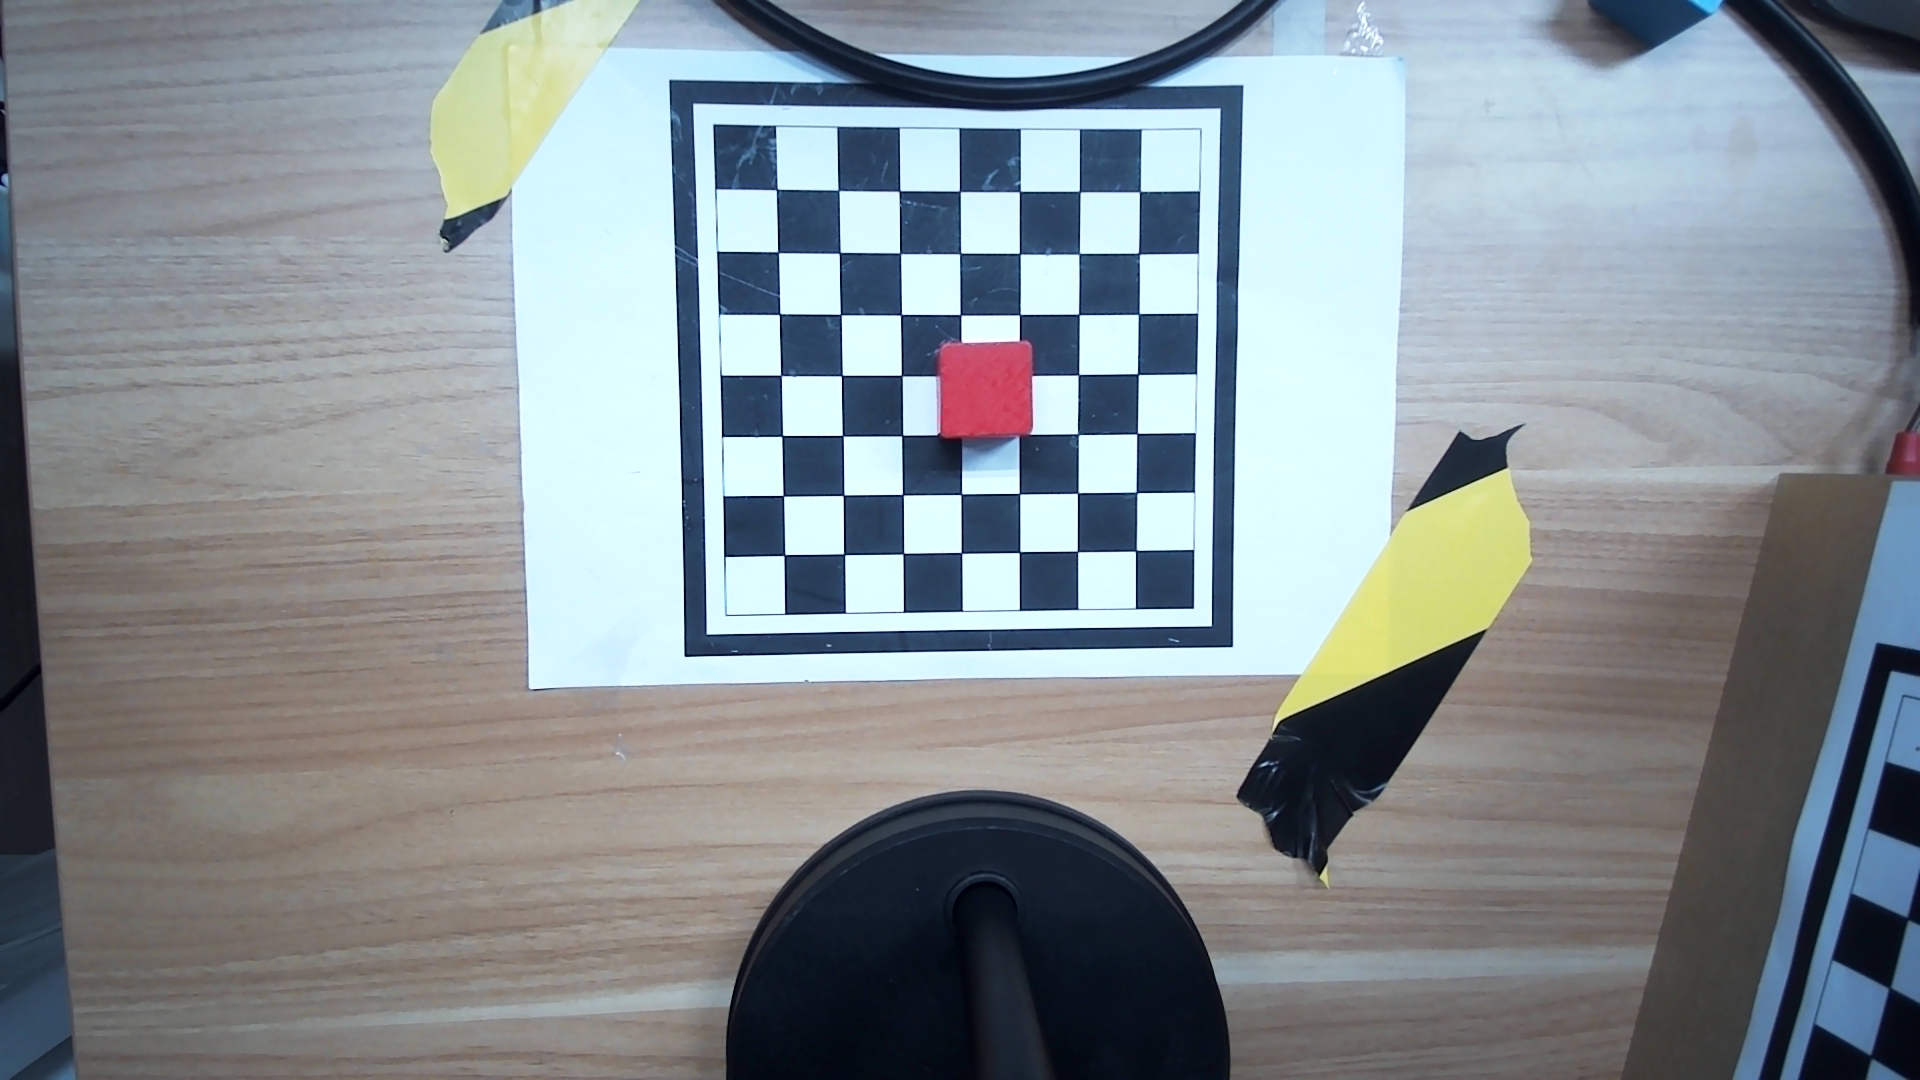
\includegraphics[width=0.72\textwidth]{task5_color_raw_image.png}
  \caption{颜色识别实验采集图像示例}
  \label{fig:task5-color-raw}
\end{figure}

\subsection{像素坐标到机械臂坐标转换}

坐标转换由 \path{daran/color_pick_place/convert.py} 实现。检测结果可以是像素点 $(u,v)$，也可以包含角度信息的字典：
\[
\{ \text{center}:(u,v),\ \text{angle}:\theta \}.
\]
转换步骤如下：

\begin{enumerate}
  \item 读取 \path{camera_calibration_result.json} 中的相机内参和畸变参数。
  \item 读取 \path{extrinsics.json} 中相机到机械臂基坐标的齐次变换 $T_{\text{robot}}^{\text{camera}}$。
  \item 使用 \texttt{cv2.undistortPoints} 将像素点转换为相机归一化射线。
  \item 将射线变换到机械臂坐标系，并与桌面平面 $z=\SI{80}{mm}$ 求交。
  \item 输出机械臂坐标 $(x,y,z)$ 和抓取姿态 $(pitch,yaw,roll)$。
\end{enumerate}

色块角度用于调整末端 yaw。程序采用 \texttt{angle\_gain=-1} 和方块角度折返函数，将图像中的平面旋转角映射到夹爪绕竖直方向的角度修正。

转换函数默认桌面高度为 \SI{80}{mm}，基础抓取姿态为 $(pitch,yaw,roll)=(0^\circ,-90^\circ,180^\circ)$。对于色块这种近似正方形目标，图像角度存在 $90^\circ$ 周期等价，因此程序使用角度折返函数将旋转修正限制在 $[-45^\circ,45^\circ)$ 内，再叠加到末端 yaw 上。这样可以避免同一个正方形目标因为 \texttt{minAreaRect} 返回角度跳变而导致夹爪姿态突变。

坐标转换是视觉抓取中最容易累积误差的环节。检测器输出的是二维像素中心，而机械臂需要的是三维空间中的抓取点。程序通过桌面平面假设将三维问题简化为射线与平面的交点计算：只要物体位于同一工作平面附近，就可以用固定高度估计抓取位置。但如果物体高度明显变化，或相机与桌面之间的外参发生移动，转换结果就会偏离真实抓取点。

像素射线与桌面平面求交的实现如代码 \ref{lst:exp5-convert-code} 所示。它先将像素点去畸变为相机归一化射线，再通过相机到机械臂坐标变换求出机器人坐标系下的桌面交点。

\lstinputlisting[
  language=Python,
  caption={像素点转换到机械臂桌面坐标的核心代码},
  label={lst:exp5-convert-code}
]{code/exp5_pixel_to_robot.py}

\subsection{抓取流程设计}

完整抓取流程由 \path{daran/color_pick_place/main.py} 实现。程序先构造检测器，再组织“识别、选择、规划、仿真、执行确认”的流程。颜色识别模式下，检测器为 \texttt{ColorBlockDetector}；程序会过滤已经在目标区域附近的物块，选择候选目标，然后构造 pick 和 place 两个 \texttt{RobotPose}。本组仅分析和仿真该流程，没有进入硬件执行。

抓取动作序列为：
\[
\text{pick\_up}\rightarrow \text{pick\_down}\rightarrow \text{pick\_up}\rightarrow
\text{transit}\rightarrow \text{place\_up}\rightarrow \text{place\_down}\rightarrow
\text{place\_up}.
\]
其中每个位姿都包含末端位置、姿态和夹爪开合状态。程序调用 \texttt{JointActionMotion.\allowbreak solve()} 将位姿动作转换为关节动作，并支持仿真预览；代码中的实机执行入口本次未使用。

程序默认 standby 关节角为 $[0,90,0,0,0,0]^\circ$，与前面实验保持一致。放置点按颜色区分：红色和黄色目标默认放在 $(180,172,90)$ mm，绿色目标放在 $(125,172,90)$ mm，蓝色目标放在 $(50,172,90)$ mm。为了避免重复搬运已经处于目标区的物块，程序设置了 \SI{40}{mm} 的目标区忽略半径；如果检测到的物块已经位于某个目标附近，则不再选择它作为待抓取对象。

抓取动作中的上方点由目标点高度加上 approach height 得到，过渡点位于较高的 transit z。这样做延续了实验三的 safe-grasp-safe 思路：视觉只负责改变抓取点的位置，运动执行仍然遵守“先上方、再下降、再抬升”的安全模板。也就是说，实验五不是把视觉结果直接发送给机械臂，而是把视觉结果嵌入一个已有的安全动作结构中。

\subsection{实验步骤与异常处理}

程序流程首先读取工作区图像，随后根据目标颜色进行分割和轮廓筛选。若检测到多个候选目标，程序会根据目标类型、位置和是否已经位于放置区域附近进行过滤。选定候选目标后，系统将像素中心转换为机械臂坐标，生成抓取上方点、抓取点、过渡点、放置上方点和放置点，最后生成仿真预览。本组没有继续执行真实动作。

异常情况主要包括未检测到目标、检测到过小轮廓、目标位于不可达区域、坐标转换失败和逆运动学求解失败。对这些情况，合理处理方式不是强行执行，而是停止当前循环、提示操作者调整光照或物体位置，并重新识别。视觉抓取系统的安全性很大程度上来自这种“识别不可靠就不执行”的保守策略。

\subsection{离线图像与程序输出分析}

图 \ref{fig:task5-visual-grasp} 展示了已有图像上锁定候选目标的离线处理结果。该图只能说明程序能够在该样例中生成目标框和中心信息，不能证明实时相机检测稳定，也不能证明机械臂能够抓取该目标。

\begin{figure}[H]
  \centering
  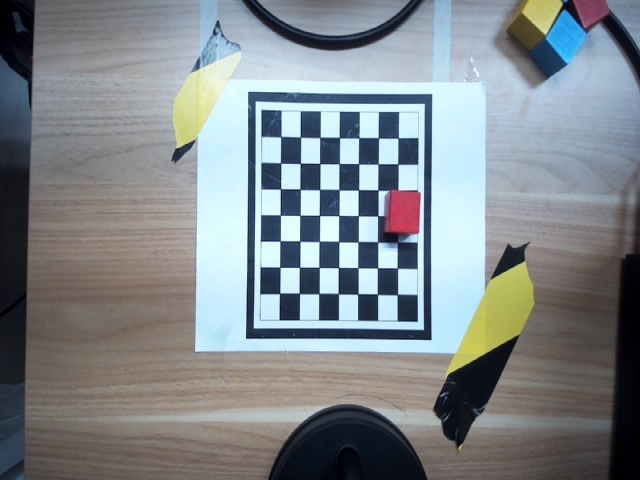
\includegraphics[width=0.72\textwidth]{task5_visual_grasp_locked.jpg}
  \caption{颜色视觉抓取目标锁定结果}
  \label{fig:task5-visual-grasp}
\end{figure}

实验中还通过人工示教建立了像素到机械臂坐标的经验仿射关系，\path{calib_result.json} 中记录的二维仿射矩阵为：
\[
\begin{bmatrix}
x_r\\y_r
\end{bmatrix}
=
\begin{bmatrix}
0.0146&0.2952&140.9101\\
0.2440&0.0154&-224.5123
\end{bmatrix}
\begin{bmatrix}
u\\v\\1
\end{bmatrix},
\]
其文件中记录的 RMS 拟合误差约为 \SI{14.10}{mm}。该数值描述已有标定点上的二维拟合残差，不等同于真实机械臂末端到达误差，且本组未通过实物抓取检验该映射。

该仿射标定共使用 12 条记录，每条记录同时保存目标颜色、机器人坐标、相机像素中心和色块角度。与实验四中的针孔模型相比，二维仿射标定更依赖示教数据本身，优点是实现简单并能吸收一部分系统性偏差，缺点是难以解释相机姿态、镜头畸变和高度变化的物理来源。对于固定相机和固定桌面的课程实验，它可以作为理论标定之外的经验补偿。

从代码结构看，颜色识别方法实现简单、计算量较小，不需要训练模型；但阈值会受到光源、背景和相机曝光参数影响。由于本组没有进行实时场景和实物抓取测试，不能判断当前阈值是否足以支持真实闭环，只能将其作为后续测试的初始参数。

本实验代码体现了视觉规划相对于固定参考点回放的潜在优势：程序可以根据图像中的目标位置重新生成 pick pose 和末端 yaw。但这一能力是否能在物体平移、旋转和光照变化下可靠工作尚未验证。此外，现有视觉识别只发生在抓取前，执行过程中没有持续视觉反馈。

\subsection{调参与鲁棒性讨论}

颜色识别方法的调参主要集中在四个方面：HSV 阈值、面积阈值、长宽比范围和形态学核大小。HSV 阈值决定哪些像素会被认为属于目标颜色；面积阈值用于过滤噪声和小反光区域；长宽比范围用于保留近似方块形状的目标；形态学核大小则影响 mask 的连通性。参数过宽会引入误检，参数过窄会导致漏检，因此需要在当前光照、背景和相机曝光条件下折中。

蓝色目标在代码中进行了额外处理：程序先对图像进行简单白平衡和饱和度增强，再在 HSV 阈值外叠加 BGR 通道约束，要求蓝色通道明显高于红色和绿色通道。绿色目标也使用类似的通道约束。这些设置是针对可能出现的暗光和反光问题设计的规则，其稳定性仍需通过不同光照条件下的图像测试确认。

颜色视觉抓取的鲁棒性边界也比较清楚：当目标颜色与背景差异明显、光照稳定、目标不遮挡时，该方法速度快、实现简单；当光照变化大、背景中存在相近颜色、目标表面反光或多个目标相互遮挡时，检测结果会变得不稳定。若误检目标进入坐标转换和运动规划，机械臂可能抓向错误位置。因此系统必须在检测不到目标、坐标转换失败或 IK 求解失败时停止，而不是继续执行。

从工程结构看，颜色识别适合作为视觉抓取代码的第一版前端，因为它可以连接“图像、坐标、规划、执行接口”各模块。实验六在此结构上保留坐标转换和抓取后端，只替换目标发现方式；两种方案的实际效果都需后续验证。

\subsection{小结}

基于颜色识别的程序完成了从图像目标、坐标转换到机械臂动作规划接口的代码连接，并生成了仿真所需的候选位姿。由于没有进行实时相机和真实机械臂验证，当前不能评价抓取成功率和环境适应性。实验六进一步在相同后端接口上引入 YOLO 检测代码。

\section{实验六：基于 YOLO 的视觉抓取}

\subsection{实验目的}

本实验在颜色视觉抓取的基础上，将目标识别部分替换为 YOLO 检测算法。实验目标不是重新编写整套抓取系统，而是保持后端坐标转换、姿态规划、IK 求解和夹爪控制不变，仅将前端目标检测器从 HSV 阈值分割替换为学习型目标检测模型。

\subsection{数据集与类别设计}

YOLO 数据位于 \texttt{daran/color\_pick\_place/yolo/}。数据集类别包含 red、green、blue 三类色块。根据 \texttt{bootstrap\_summary.json}，数据集中共有 213 张图像、1041 个标注框，各类别数量如表 \ref{tab:yolo-dataset} 所示。

\begin{table}[H]
  \centering
  \caption{YOLO 数据集统计}
  \label{tab:yolo-dataset}
  \begin{tabular}{lcc}
    \toprule
    类别 & 标注框数量 & 占比 \\
    \midrule
    red & 391 & 37.6\% \\
    green & 320 & 30.7\% \\
    blue & 330 & 31.7\% \\
    \midrule
    合计 & 1041 & 100\% \\
    \bottomrule
  \end{tabular}
\end{table}

\texttt{data.yaml} 指定训练集和验证集目录，并定义类别名称。需要注意的是，该文件中的数据集路径为原训练机器上的绝对路径，因此在不同机器上复现实验时需要将 \texttt{path} 改为当前仓库下的实际路径。

\subsection{YOLO 模型训练与推理}

训练脚本为 \texttt{daran/color\_pick\_place/yolo/train.py}。程序从 \texttt{yolo11n.pt} 初始化模型，训练 120 个 epoch，输入尺寸为 960，batch size 为 16。由于类别本身就是颜色，训练脚本中特意设置 \texttt{hsv\_h=0.0}，避免色相增强把红色样本扰动成橙色或其它颜色，从而破坏类别标签。几何增强则保持较强，包括 \SI{180}{\degree} 旋转、水平/垂直翻转、平移、缩放和 mosaic。

最终训练结果位于 \texttt{runs/blocks/}，权重文件包括 \texttt{best.pt} 和 \texttt{last.pt}。训练曲线和混淆矩阵如图 \ref{fig:task6-training} 和图 \ref{fig:task6-confusion} 所示。最后一个 epoch 的验证指标约为 precision=0.9917、recall=0.9922、mAP50=0.9915、mAP50--95=0.8577。

\begin{figure}[H]
  \centering
  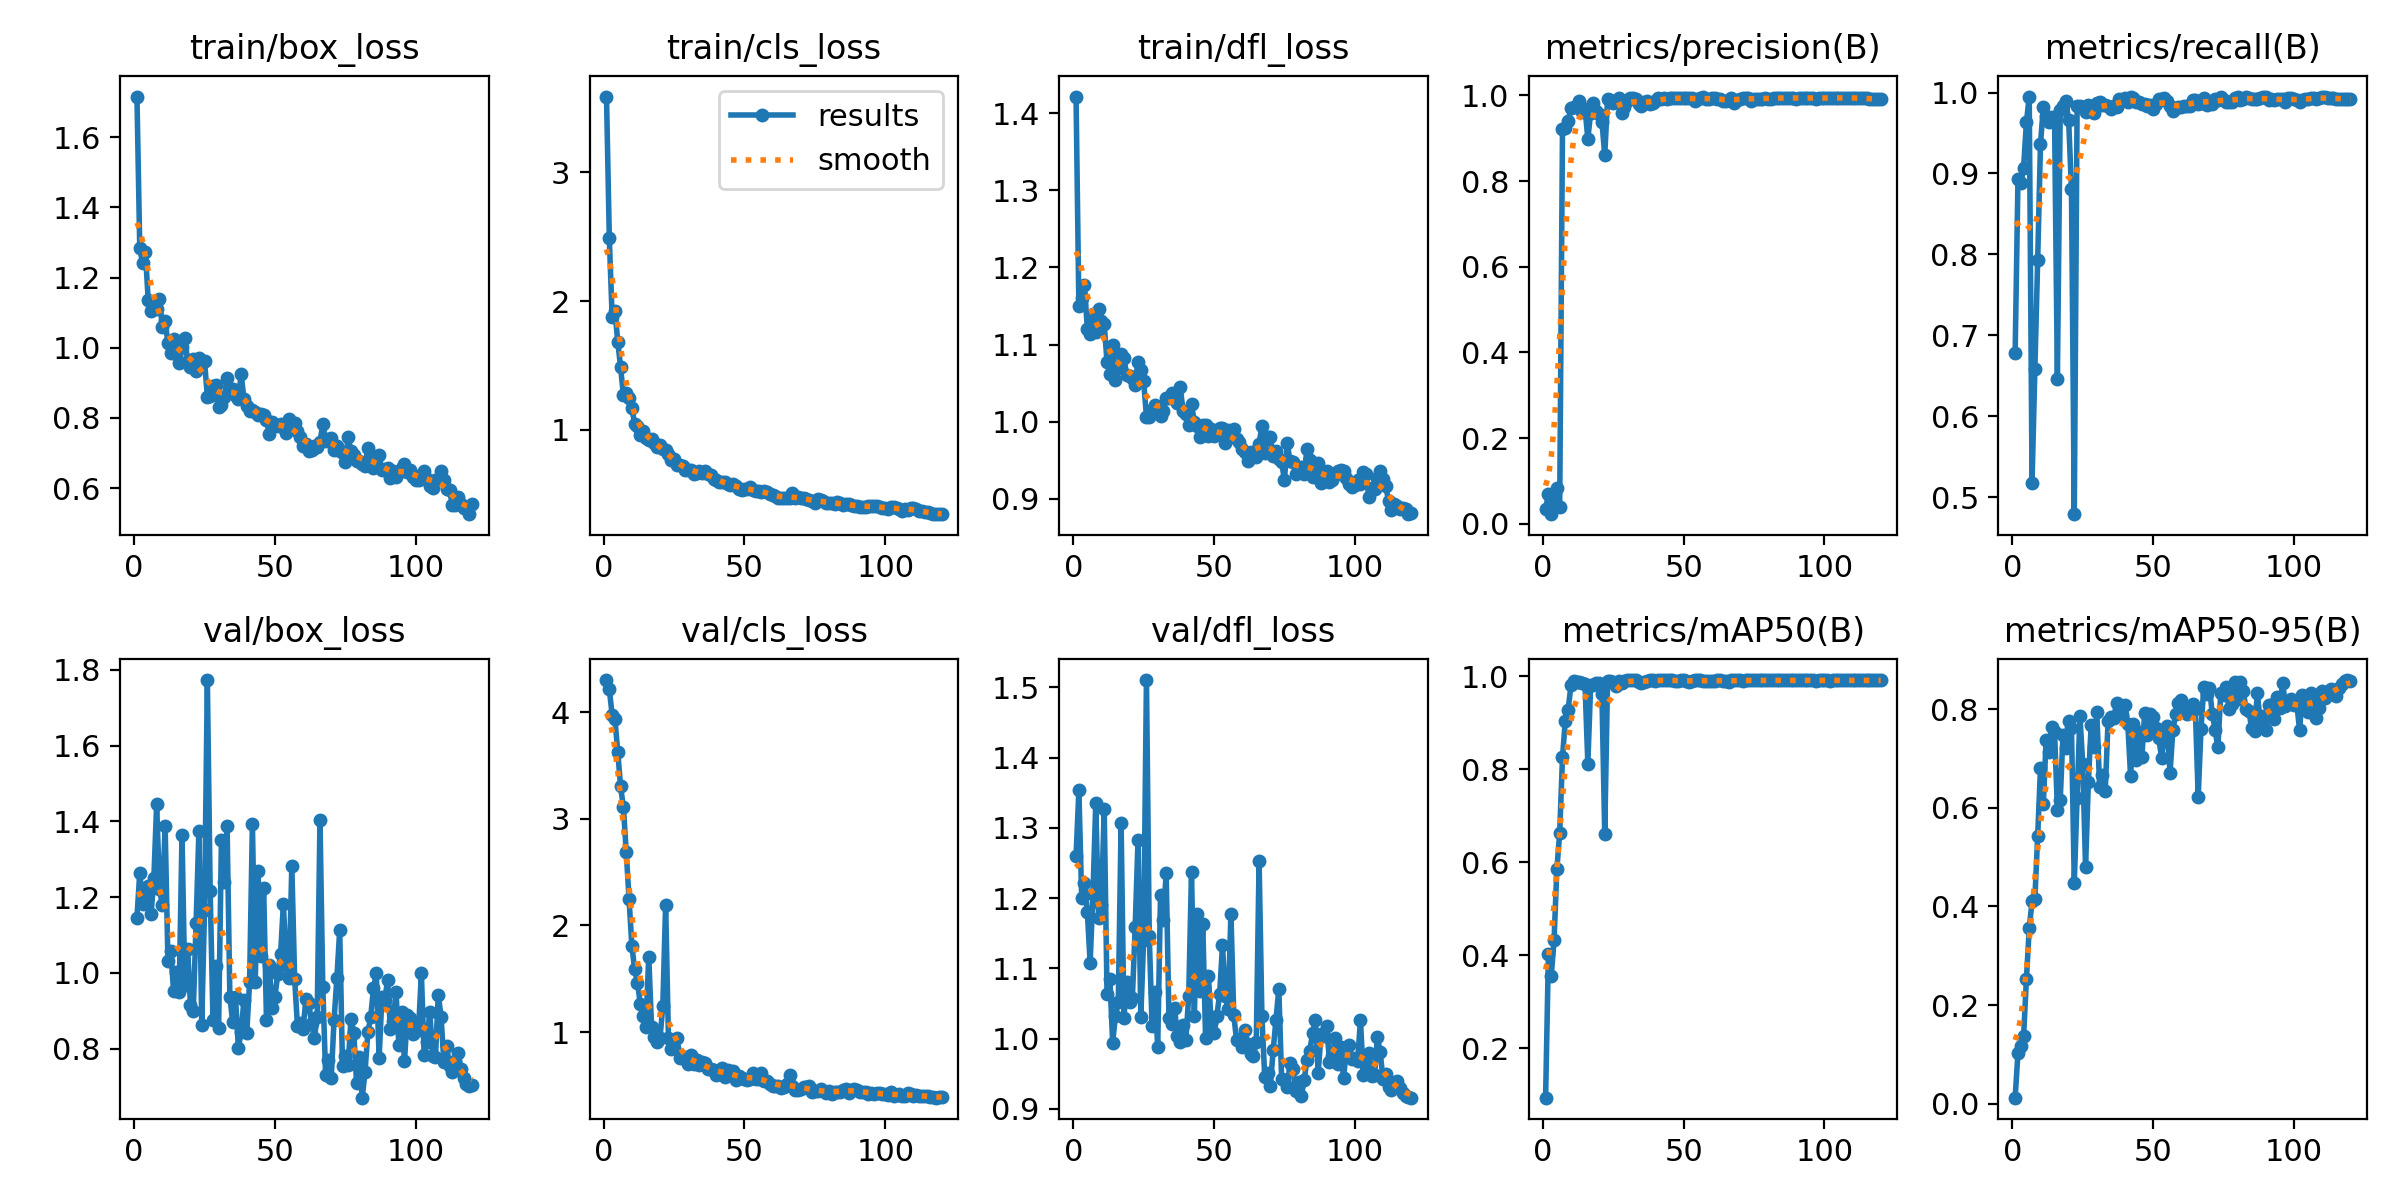
\includegraphics[width=0.82\textwidth]{task6_yolo_training_results.png}
  \caption{YOLO 训练指标曲线}
  \label{fig:task6-training}
\end{figure}

\begin{figure}[H]
  \centering
  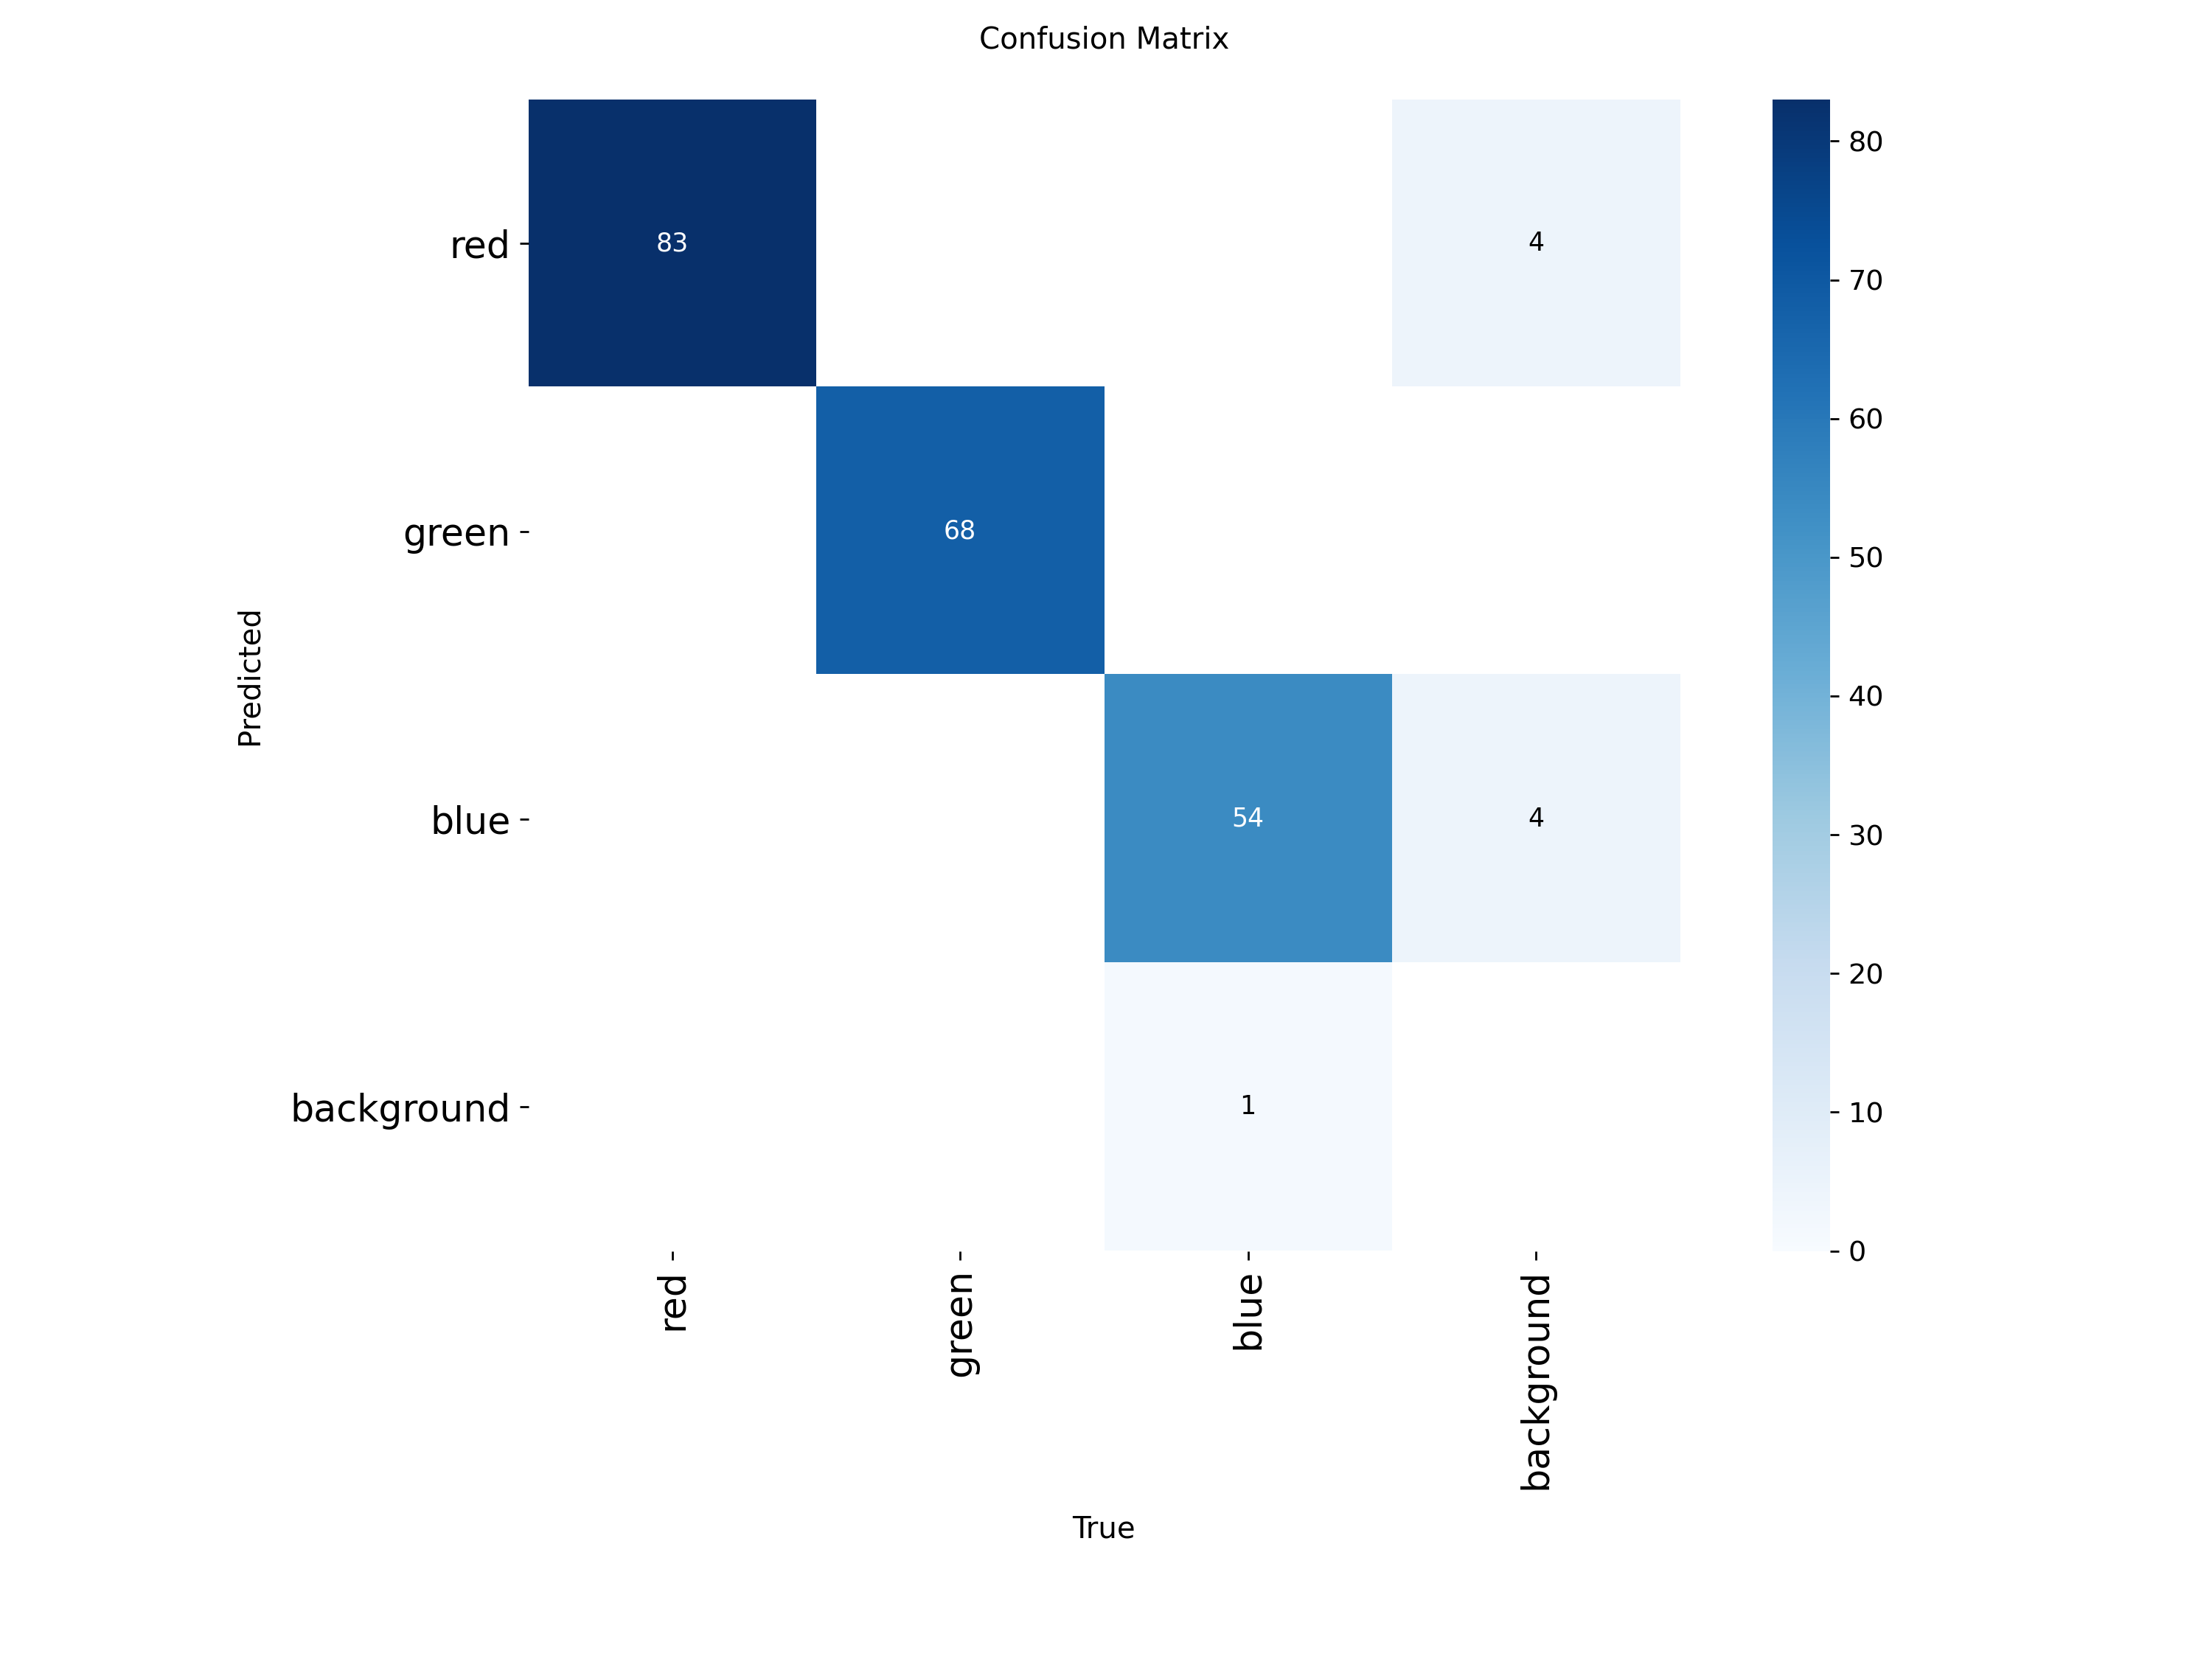
\includegraphics[width=0.68\textwidth]{task6_yolo_confusion_matrix.png}
  \caption{YOLO 验证集混淆矩阵}
  \label{fig:task6-confusion}
\end{figure}

\subsection{与颜色识别方法的接口复用}

YOLO 检测器实现于 \texttt{daran/color\_pick\_place/yolo/yolo\_detector.py}。该模块被设计为与 \texttt{ColorBlockDetector} 兼容，二者都提供：

\begin{lstlisting}[language=Python,caption={检测器接口约定}]
recognize() -> [{"type": str, "center": (u, v), "angle": float}, ...]
release()
\end{lstlisting}

因此 \texttt{main.py} 中只需通过参数选择 \texttt{--detector yolo} 或 \texttt{--detector color}，后续 \texttt{camera\_observation\_to\_robot\_pose()}、目标筛选、抓取动作构造和运动执行均可复用。

YOLO 检测器的一个关键设计是：YOLO 负责给出目标类别和边界框，随后仍在检测框 ROI 内调用原颜色 mask 和 \texttt{cv2.minAreaRect} 细化中心点和角度。这样做保留了旧系统对 \texttt{center} 和 \texttt{angle} 的定义，避免后端抓取姿态映射重新标定。

\subsection{实验结果与对比分析}

图 \ref{fig:task6-parity} 展示了 YOLO 检测和原有颜色逻辑对齐检查的结果。相比颜色阈值方法，YOLO 能利用目标形状、上下文和训练样本分布，在光照变化、局部阴影和颜色接近背景时更稳定；但 YOLO 也引入了训练数据、标注质量、模型权重和推理设备依赖。

\begin{figure}[H]
  \centering
  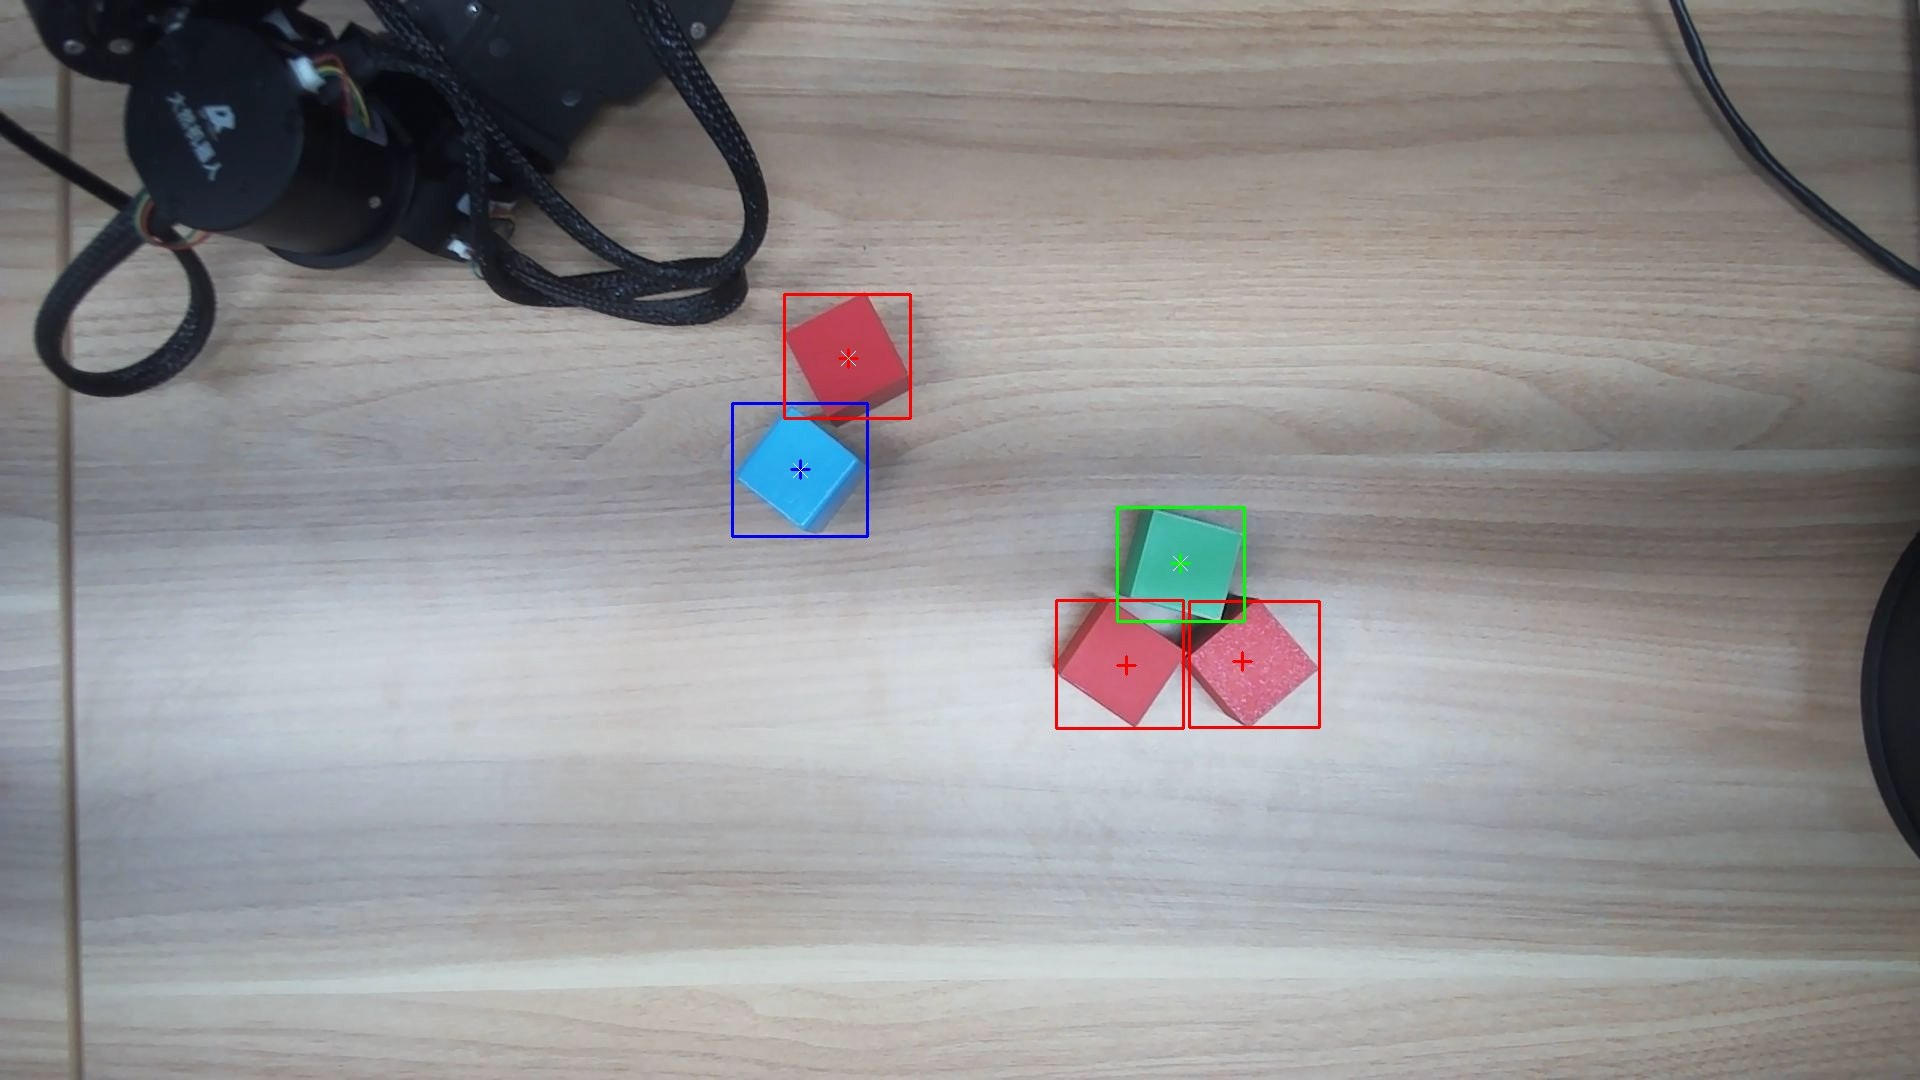
\includegraphics[width=0.76\textwidth]{task6_yolo_parity_overlay.jpg}
  \caption{YOLO 检测结果与颜色逻辑对齐检查}
  \label{fig:task6-parity}
\end{figure}

\begin{table}[H]
  \centering
  \caption{颜色识别与 YOLO 识别对比}
  \label{tab:color-yolo-compare}
  \begin{tabular}{lll}
    \toprule
    项目 & 颜色阈值识别 & YOLO 识别 \\
    \midrule
    前期成本 & 无需训练，调阈值即可 & 需要采集、标注和训练数据 \\
    推理速度 & 很快，CPU 即可 & 取决于模型和设备 \\
    光照适应性 & 较弱，需调 HSV 阈值 & 较强，依赖训练集覆盖 \\
    可扩展性 & 类别增多后阈值维护困难 & 可通过新增类别和再训练扩展 \\
    与抓取接口 & 直接输出中心和角度 & 输出框后再细化中心和角度 \\
    \bottomrule
  \end{tabular}
\end{table}

\subsection{小结}

本实验完成了视觉识别模块的算法升级。通过保持检测器输出接口一致，YOLO 能够无缝接入原有抓取系统，使实验五中的坐标转换、轨迹规划和夹爪控制继续复用。该设计体现了良好的模块边界：感知前端可以替换，运动控制后端保持稳定。

\section{总结与展望}

\subsection{实验总结}

本学期六组实验从基础环境配置开始，逐步完成机械臂运动控制、抓取搬运、相机标定和视觉引导抓取。整体技术路线可以概括为：

\[
\begin{aligned}
\text{环境配置}&\rightarrow \text{运动学建模}\rightarrow \text{轨迹规划}\\
&\rightarrow \text{抓取动作}\rightarrow \text{相机标定}
\rightarrow \text{视觉识别}\rightarrow \text{视觉抓取}.
\end{aligned}
\]

实验一完成了 Python、Robotics Toolbox、OpenCV、串口通信等基础环境配置；实验二建立 DH 模型并实现末端直线运动；实验三在示教点基础上完成抓取搬运；实验四通过棋盘格标定获得相机内参、畸变参数和工作平面坐标关系；实验五使用颜色分割完成目标定位和视觉抓取；实验六使用 YOLO 替代颜色阈值识别，提高了视觉前端的鲁棒性和可扩展性。

\subsection{误差来源分析}

综合各实验，系统误差主要来自以下几个方面：

\begin{itemize}
  \item \textbf{运动学模型误差：} DH 参数与真实机械臂结构之间存在制造和装配误差，舵机零位也可能与模型零位不完全一致。
  \item \textbf{执行机构误差：} 一体化关节存在回差、摩擦和负载扰动，夹爪闭合宽度也会受物体材质影响。
  \item \textbf{相机标定误差：} 棋盘格角点检测、相机固定稳定性、工作平面高度假设都会影响像素到世界坐标的转换。
  \item \textbf{视觉检测误差：} 颜色阈值受光照影响明显，YOLO 检测则依赖训练数据覆盖范围和标注质量。
  \item \textbf{任务规划误差：} 抓取高度、下降距离、目标角度估计和放置点高度若设置不合理，会导致抓取不稳或放置偏差。
\end{itemize}

\subsection{改进方向}

后续可以从以下方向继续完善系统：

\begin{enumerate}
  \item 增加手眼标定流程，减少相机坐标到机械臂基坐标之间的人工标定误差。
  \item 在抓取前加入二次视觉确认，检测物体是否在夹爪正下方。
  \item 引入深度相机或多视角测量，避免单平面高度假设带来的误差。
  \item 扩充 YOLO 数据集，加入不同光照、遮挡、背景和物体姿态。
  \item 将轨迹规划从关键点插值升级为带速度、加速度约束的更平滑规划。
  \item 在真实执行中记录关节反馈和末端误差，形成闭环校正机制。
\end{enumerate}

总体来看，本实验已经形成了一个可运行、可扩展的桌面机械臂视觉抓取系统。它的核心价值不只是完成单个抓取动作，而是建立了从感知、坐标转换、运动规划到执行控制的完整链路，为后续更复杂的自主操作任务打下基础。


\nocite{opencv,roboticstoolbox,ultralytics}
\bibliographystyle{plain}
\bibliography{references}

% \appendix
% \clearpage
\section{完整实验代码}

本附录收录本学期实验报告对应的完整代码。为便于报告独立编译，代码文件已整理至 \codepath{report/code/appendix/} 目录；其中 Jupyter Notebook 按代码单元导出为 Python 文件。

\subsection{实验一：环境配置}

\lstinputlisting[style=appendixcode,caption={environment.yml}]{code/appendix/env/environment.yml}

\subsection{实验二：机械臂末端直线运动}

\lstinputlisting[style=appendixcode,language=Python,caption={dh\_cartesian\_line\_motion.py}]{code/appendix/task1/dh_cartesian_line_motion.py}

\lstinputlisting[style=appendixcode,language=Python,caption={dh\_roboticstoolbox\_control.py}]{code/appendix/task1/dh_roboticstoolbox_control.py}

\lstinputlisting[style=appendixcode,language=Python,caption={arm\_gui\_control.py}]{code/appendix/task1/arm_gui_control.py}

\lstinputlisting[style=appendixcode,language=Python,caption={visualize\_zero\_pose.py}]{code/appendix/task1/visualize_zero_pose.py}

\lstinputlisting[style=appendixcode,language=Python,caption={visualize\_park\_pose.py}]{code/appendix/task1/visualize_park_pose.py}

\lstinputlisting[style=appendixcode,language=Python,caption={debug\_gripper.py}]{code/appendix/task1/debug_gripper.py}

\subsection{实验三：机械臂抓取与搬运}

\lstinputlisting[style=appendixcode,language=Python,caption={pick\_and\_place.py}]{code/appendix/task2/pick_and_place.py}

\subsection{实验四：相机标定与坐标投影}

\lstinputlisting[style=appendixcode,language=Python,caption={camera\_calibration.py}]{code/appendix/task3/camera_calibration.py}

\lstinputlisting[style=appendixcode,language=Python,caption={pose\_projection.py}]{code/appendix/task3/pose_projection.py}

\lstinputlisting[style=appendixcode,language=Python,caption={auto\_calib.py}]{code/appendix/color_pick_place/auto_calib.py}

\lstinputlisting[style=appendixcode,language=Python,caption={manual\_calib.py}]{code/appendix/color_pick_place/manual_calib.py}

\lstinputlisting[style=appendixcode,language=Python,caption={teach\_calib.py}]{code/appendix/color_pick_place/teach_calib.py}

\lstinputlisting[style=appendixcode,language=Python,caption={calibrate\_intrinsics.py}]{code/appendix/color_pick_place/calibrate_intrinsics.py}

\lstinputlisting[style=appendixcode,language=Python,caption={calc\_extrinsics.py}]{code/appendix/color_pick_place/calc_extrinsics.py}

\subsection{实验五：基于颜色识别的视觉抓取}

\lstinputlisting[style=appendixcode,language=Python,caption={visual\_grasp.py}]{code/appendix/task3/visual_grasp.py}

\lstinputlisting[style=appendixcode,language=Python,caption={main.py}]{code/appendix/color_pick_place/main.py}

\lstinputlisting[style=appendixcode,language=Python,caption={detect.py}]{code/appendix/color_pick_place/detect.py}

\lstinputlisting[style=appendixcode,language=Python,caption={convert.py}]{code/appendix/color_pick_place/convert.py}

\subsection{实验六：基于 YOLO 的视觉识别与抓取}

\lstinputlisting[style=appendixcode,language=Python,caption={yolo\_detector.py}]{code/appendix/color_pick_place/yolo/yolo_detector.py}

\lstinputlisting[style=appendixcode,language=Python,caption={train.py}]{code/appendix/color_pick_place/yolo/train.py}

\lstinputlisting[style=appendixcode,language=Python,caption={validate\_detector.py}]{code/appendix/color_pick_place/yolo/validate_detector.py}

\lstinputlisting[style=appendixcode,language=Python,caption={bootstrap\_labels.py}]{code/appendix/color_pick_place/yolo/bootstrap_labels.py}

\lstinputlisting[style=appendixcode,language=Python,caption={make\_split.py}]{code/appendix/color_pick_place/yolo/make_split.py}

\lstinputlisting[style=appendixcode,caption={data.yaml}]{code/appendix/color_pick_place/yolo/data.yaml}

\lstinputlisting[style=appendixcode,caption={classes.txt}]{code/appendix/color_pick_place/yolo/classes.txt}

\subsection{底层控制与公共工具代码}

\lstinputlisting[style=appendixcode,language=Python,caption={arm\_robot.py}]{code/appendix/color_pick_place/arm_robot.py}

\lstinputlisting[style=appendixcode,language=Python,caption={arm\_six\_axis.py}]{code/appendix/color_pick_place/arm_six_axis.py}

\lstinputlisting[style=appendixcode,language=Python,caption={DrEmpower\_can.py}]{code/appendix/color_pick_place/DrEmpower_can.py}

\lstinputlisting[style=appendixcode,language=Python,caption={gripper.py}]{code/appendix/color_pick_place/gripper.py}

\lstinputlisting[style=appendixcode,language=Python,caption={joint\_action\_motion.py}]{code/appendix/color_pick_place/joint_action_motion.py}

\lstinputlisting[style=appendixcode,language=Python,caption={parameter\_interface.py}]{code/appendix/color_pick_place/parameter_interface.py}

\lstinputlisting[style=appendixcode,language=Python,caption={umatrix.py}]{code/appendix/color_pick_place/umatrix.py}


\end{document}
